% RCMLR 2026 workshop submission -- "What a median alert lead time measures: a reporting
% gap in continuously evaluated clinical models". The title lives here AND in PAPER.md front matter; keep them
% in step, build_tex.py does not sync it.
%
% TEMPLATE: neurips_2026.sty, the official style file, fetched from
% https://media.neurips.cc/Conferences/NeurIPS2026/Formatting_Instructions_For_NeurIPS_2026.zip
% (CC BY 4.0). Its option interface is identical to the 2025 file: `dblblindworkshop`,
% `sglblindworkshop`, `final`, `preprint`, `nonatbib`, and \workshoptitle.
%
% ANONYMITY: the review is DOUBLE-BLIND (confirmed by the author, 2026-08-28), so
% `dblblindworkshop` is correct and stays. It keeps \@anonymous true, so the \author block
% below is ignored and the title page prints the anonymous placeholders instead. Do not
% switch to `sglblindworkshop` for the review copy; that is the camera-ready change.
\documentclass{article}
\usepackage[dblblindworkshop]{neurips_2026}
\workshoptitle{Responsible Communication of Machine Learning Research in Biomedicine}

\usepackage[utf8]{inputenc}
\usepackage[T1]{fontenc}
% hidelinks: plain hyperref draws a coloured border box around every link, which prints as
% a rectangle over each citation and reference. The links stay live, they just stop being
% framed. Set here rather than in neurips_2026.sty, which stays as shipped.
\usepackage[hidelinks]{hyperref}
\usepackage{url}
\usepackage{booktabs}
\usepackage{amsmath}
\usepackage{amssymb}
\usepackage{graphicx}
\usepackage{longtable}
\usepackage{array}
\usepackage{calc}
\usepackage{microtype}
% The checklist's answer macros in neurips_2026.sty use \textcolor; the style file itself
% does not load a colour package.
\usepackage{xcolor}
% [H] for the appendix exhibits, which must stay under their own headings.
\usepackage{float}

% pandoc emits these for its table and list output.
\providecommand{\tightlist}{%
  \setlength{\itemsep}{0pt}\setlength{\parskip}{0pt}}
\newlength{\cslhangindent}
\setlength{\cslhangindent}{1.5em}
\providecommand{\pandocbounded}[1]{#1}

% Table 1 is dense; give it room without shrinking the body text.
\usepackage{etoolbox}
\AtBeginEnvironment{longtable}{\footnotesize}

% The style file builds a workshop-aware notice from \workshoptitle, but only reaches for it
% under `final'. Under `dblblindworkshop' it emits the generic main-track notice instead, which
% names a conference this paper was not submitted to. Restate the notice here rather than editing
% neurips_2026.sty, which stays as shipped.
\makeatletter
\renewcommand{\@noticestring}{%
  Submitted to the NeurIPS \@neuripsyear\ Workshop on \@workshoptitle. Do not distribute.%
}
\makeatother

\graphicspath{{../}}

\title{What a median alert lead time measures: a reporting gap in continuously evaluated clinical models}

% Anonymous under dblblindworkshop; this block is ignored until the option is
% changed to sglblindworkshop.
\author{%
  Anonymous Author(s) \\
  Affiliation \\
  \texttt{email}
}

\begin{document}
\maketitle

% ORDER: body, references, appendix, checklist. This is the order the official
% neurips_2026.tex demonstrates (\section*{References}, then \appendix, then
% \section*{NeurIPS Paper Checklist}



\begin{enumerate}

\item {\bf Claims}
    \item[] Question: Do the main claims made in the abstract and introduction accurately reflect the paper's contributions and scope?
    \item[] Answer: \answerYes{}
    \item[] Justification: The abstract and Section 1 state the four contributions and their scope. They distinguish the observed lead--window association from what the upward-biased shuffle can establish, treat low directedness as descriptive rather than causal, and state that the paper measures neither clinician comprehension nor physiology.
    \item[] Guidelines:
    \begin{itemize}
        \item The answer \answerNA{} means that the abstract and introduction do not include the claims made in the paper.
        \item The abstract and/or introduction should clearly state the claims made, including the contributions made in the paper and important assumptions and limitations. A \answerNo{} or \answerNA{} answer to this question will not be perceived well by the reviewers. 
        \item The claims made should match theoretical and experimental results, and reflect how much the results can be expected to generalize to other settings. 
        \item It is fine to include aspirational goals as motivation as long as it is clear that these goals are not attained by the paper. 
    \end{itemize}

\item {\bf Limitations}
    \item[] Question: Does the paper discuss the limitations of the work performed by the authors?
    \item[] Answer: \answerYes{}
    \item[] Justification: Section 7 is a separate limitations section covering the retrospective design, the single outcome definition, single training seed and operating-point family, the pipeline-specific results, null selection and upward bias, the single clinical domain, and the unvalidated communication and reporting proposals.
    \item[] Guidelines:
    \begin{itemize}
        \item The answer \answerNA{} means that the paper has no limitation while the answer \answerNo{} means that the paper has limitations, but those are not discussed in the paper. 
        \item The authors are encouraged to create a separate ``Limitations'' section in their paper.
        \item The paper should point out any strong assumptions and how robust the results are to violations of these assumptions (e.g., independence assumptions, noiseless settings, model well-specification, asymptotic approximations only holding locally). The authors should reflect on how these assumptions might be violated in practice and what the implications would be.
        \item The authors should reflect on the scope of the claims made, e.g., if the approach was only tested on a few datasets or with a few runs. In general, empirical results often depend on implicit assumptions, which should be articulated.
        \item The authors should reflect on the factors that influence the performance of the approach. For example, a facial recognition algorithm may perform poorly when image resolution is low or images are taken in low lighting. Or a speech-to-text system might not be used reliably to provide closed captions for online lectures because it fails to handle technical jargon.
        \item The authors should discuss the computational efficiency of the proposed algorithms and how they scale with dataset size.
        \item If applicable, the authors should discuss possible limitations of their approach to address problems of privacy and fairness.
        \item While the authors might fear that complete honesty about limitations might be used by reviewers as grounds for rejection, a worse outcome might be that reviewers discover limitations that aren't acknowledged in the paper. The authors should use their best judgment and recognize that individual actions in favor of transparency play an important role in developing norms that preserve the integrity of the community. Reviewers will be specifically instructed to not penalize honesty concerning limitations.
    \end{itemize}

\item {\bf Theory assumptions and proofs}
    \item[] Question: For each theoretical result, does the paper provide the full set of assumptions and a complete (and correct) proof?
    \item[] Answer: \answerNA{}
    \item[] Justification: The paper contains no theorems, lemmas or formal results. Its claims are empirical and each is measured on cached scores.
    \item[] Guidelines:
    \begin{itemize}
        \item The answer \answerNA{} means that the paper does not include theoretical results. 
        \item All the theorems, formulas, and proofs in the paper should be numbered and cross-referenced.
        \item All assumptions should be clearly stated or referenced in the statement of any theorems.
        \item The proofs can either appear in the main paper or the supplemental material, but if they appear in the supplemental material, the authors are encouraged to provide a short proof sketch to provide intuition. 
        \item Inversely, any informal proof provided in the core of the paper should be complemented by formal proofs provided in appendix or supplemental material.
        \item Theorems and Lemmas that the proof relies upon should be properly referenced. 
    \end{itemize}

    \item {\bf Experimental result reproducibility}
    \item[] Question: Does the paper fully disclose all the information needed to reproduce the main experimental results of the paper to the extent that it affects the main claims and/or conclusions of the paper (regardless of whether the code and data are provided or not)?
    \item[] Answer: \answerYes{}
    \item[] Justification: Yes. Two standards should be distinguished. Independent reimplementation is supported: Section 2 gives the task, cohorts, scoring policy and alert rule; Appendix A.1 gives the split sizes and seed, the eligibility rules, the twenty inputs and how each family consumes them, every architecture and training hyperparameter, and the software versions; Appendix A.19 records the seeds and resampling counts; both datasets are available under their providers' access procedures; and the analysis code is released at the anonymized repository Appendix A.1 names. Bit-for-bit reproduction from raw data is not supported here, because neither dataset may be redistributed and the cached per-minute scores the analyses read are derived patient-level data governed by the same agreements, so they are not in the repository and a reader must obtain the data themselves. We claim the first and not the second.
    \item[] Guidelines:
    \begin{itemize}
        \item The answer \answerNA{} means that the paper does not include experiments.
        \item If the paper includes experiments, a \answerNo{} answer to this question will not be perceived well by the reviewers: Making the paper reproducible is important, regardless of whether the code and data are provided or not.
        \item If the contribution is a dataset and\slash or model, the authors should describe the steps taken to make their results reproducible or verifiable. 
        \item Depending on the contribution, reproducibility can be accomplished in various ways. For example, if the contribution is a novel architecture, describing the architecture fully might suffice, or if the contribution is a specific model and empirical evaluation, it may be necessary to either make it possible for others to replicate the model with the same dataset, or provide access to the model. In general. releasing code and data is often one good way to accomplish this, but reproducibility can also be provided via detailed instructions for how to replicate the results, access to a hosted model (e.g., in the case of a large language model), releasing of a model checkpoint, or other means that are appropriate to the research performed.
        \item While NeurIPS does not require releasing code, the conference does require all submissions to provide some reasonable avenue for reproducibility, which may depend on the nature of the contribution. For example
        \begin{enumerate}
            \item If the contribution is primarily a new algorithm, the paper should make it clear how to reproduce that algorithm.
            \item If the contribution is primarily a new model architecture, the paper should describe the architecture clearly and fully.
            \item If the contribution is a new model (e.g., a large language model), then there should either be a way to access this model for reproducing the results or a way to reproduce the model (e.g., with an open-source dataset or instructions for how to construct the dataset).
            \item We recognize that reproducibility may be tricky in some cases, in which case authors are welcome to describe the particular way they provide for reproducibility. In the case of closed-source models, it may be that access to the model is limited in some way (e.g., to registered users), but it should be possible for other researchers to have some path to reproducing or verifying the results.
        \end{enumerate}
    \end{itemize}


\item {\bf Open access to data and code}
    \item[] Question: Does the paper provide open access to the data and code, with sufficient instructions to faithfully reproduce the main experimental results, as described in supplemental material?
    \item[] Answer: \answerYes{}
    \item[] Justification: The analysis code is released at an anonymized repository under the Apache License 2.0, which Appendix A.1 names, together with the aggregate result files behind every table and figure, so the table and figure checks run from the repository as shipped. The datasets are not redistributed there and cannot be: VitalDB is under a Creative Commons Attribution-NonCommercial-ShareAlike 4.0 International license and a data use agreement and MOVER is under a data use agreement, and the cached per-minute scores are derived patient-level data governed by the same agreements. Both are obtained from their own project sites once access is granted, as Appendix A.1 records, and Appendix A.1 specifies the construction to the level a reimplementation needs.
    \item[] Guidelines:
    \begin{itemize}
        \item The answer \answerNA{} means that paper does not include experiments requiring code.
        \item Please see the NeurIPS code and data submission guidelines (\url{https://neurips.cc/public/guides/CodeSubmissionPolicy}) for more details.
        \item While we encourage the release of code and data, we understand that this might not be possible, so \answerNo{} is an acceptable answer. Papers cannot be rejected simply for not including code, unless this is central to the contribution (e.g., for a new open-source benchmark).
        \item The instructions should contain the exact command and environment needed to run to reproduce the results. See the NeurIPS code and data submission guidelines (\url{https://neurips.cc/public/guides/CodeSubmissionPolicy}) for more details.
        \item The authors should provide instructions on data access and preparation, including how to access the raw data, preprocessed data, intermediate data, and generated data, etc.
        \item The authors should provide scripts to reproduce all experimental results for the new proposed method and baselines. If only a subset of experiments are reproducible, they should state which ones are omitted from the script and why.
        \item At submission time, to preserve anonymity, the authors should release anonymized versions (if applicable).
        \item Providing as much information as possible in supplemental material (appended to the paper) is recommended, but including URLs to data and code is permitted.
    \end{itemize}


\item {\bf Experimental setting/details}
    \item[] Question: Does the paper specify all the training and test details (e.g., data splits, hyperparameters, how they were chosen, type of optimizer) necessary to understand the results?
    \item[] Answer: \answerYes{}
    \item[] Justification: Appendix A.1 gives the subject-aware split and its sizes, the seed, the per-minute eligibility rules, the feature set, and for each of the five families the architecture, optimizer, learning rate, weight decay, batch size, epoch budget and early-stopping rule. Section 2 gives the calibration and threshold policy: fitted on the development validation split at an 80\% case-level sensitivity target and transported unchanged, with nothing reselected.
    \item[] Guidelines:
    \begin{itemize}
        \item The answer \answerNA{} means that the paper does not include experiments.
        \item The experimental setting should be presented in the core of the paper to a level of detail that is necessary to appreciate the results and make sense of them.
        \item The full details can be provided either with the code, in appendix, or as supplemental material.
    \end{itemize}

\item {\bf Experiment statistical significance}
    \item[] Question: Does the paper report error bars suitably and correctly defined or other appropriate information about the statistical significance of the experiments?
    \item[] Answer: \answerYes{}
    \item[] Justification: Every interval in the paper is a 95\% cluster bootstrap on the clustering unit named in Section 2, the subject for two cohorts and the case for MOVER (SIS), at 2,000 replicates; permutation nulls use 1,000 replicates and are reported as the 2.5th and 97.5th percentiles of the null distribution rather than as symmetric error bars. Appendix A.18 records the multiplicity family and its Benjamini--Hochberg adjustment, and Appendix A.19 the seeds.
    \item[] Guidelines:
    \begin{itemize}
        \item The answer \answerNA{} means that the paper does not include experiments.
        \item The authors should answer \answerYes{} if the results are accompanied by error bars, confidence intervals, or statistical significance tests, at least for the experiments that support the main claims of the paper.
        \item The factors of variability that the error bars are capturing should be clearly stated (for example, train/test split, initialization, random drawing of some parameter, or overall run with given experimental conditions).
        \item The method for calculating the error bars should be explained (closed form formula, call to a library function, bootstrap, etc.)
        \item The assumptions made should be given (e.g., Normally distributed errors).
        \item It should be clear whether the error bar is the standard deviation or the standard error of the mean.
        \item It is OK to report 1-sigma error bars, but one should state it. The authors should preferably report a 2-sigma error bar than state that they have a 96\% CI, if the hypothesis of Normality of errors is not verified.
        \item For asymmetric distributions, the authors should be careful not to show in tables or figures symmetric error bars that would yield results that are out of range (e.g., negative error rates).
        \item If error bars are reported in tables or plots, the authors should explain in the text how they were calculated and reference the corresponding figures or tables in the text.
    \end{itemize}

\item {\bf Experiments compute resources}
    \item[] Question: For each experiment, does the paper provide sufficient information on the computer resources (type of compute workers, memory, time of execution) needed to reproduce the experiments?
    \item[] Answer: \answerYes{}
    \item[] Justification: Appendix A.1 reports the hardware (one Apple M3 Ultra desktop with 512 GB unified memory, PyTorch on the Metal backend, no GPU cluster), the wall clock for each of the five models, and the fact that the project trained more than the paper reports, namely a seven-point lead-time sweep per family. The analyses in this paper add no training and read cached scores.
    \item[] Guidelines:
    \begin{itemize}
        \item The answer \answerNA{} means that the paper does not include experiments.
        \item The paper should indicate the type of compute workers CPU or GPU, internal cluster, or cloud provider, including relevant memory and storage.
        \item The paper should provide the amount of compute required for each of the individual experimental runs as well as estimate the total compute. 
        \item The paper should disclose whether the full research project required more compute than the experiments reported in the paper (e.g., preliminary or failed experiments that didn't make it into the paper). 
    \end{itemize}
    
\item {\bf Code of ethics}
    \item[] Question: Does the research conducted in the paper conform, in every respect, with the NeurIPS Code of Ethics \url{https://neurips.cc/public/EthicsGuidelines}?
    \item[] Answer: \answerYes{}
    \item[] Justification: The research conforms to the NeurIPS Code of Ethics. It is a secondary analysis of de-identified data obtained under the providers' data use agreements, with an institutional review board exemption and consent waiver recorded in Section 2 and Appendix A.1, and it proposes no model for clinical use.
    \item[] Guidelines:
    \begin{itemize}
        \item The answer \answerNA{} means that the authors have not reviewed the NeurIPS Code of Ethics.
        \item If the authors answer \answerNo, they should explain the special circumstances that require a deviation from the Code of Ethics.
        \item The authors should make sure to preserve anonymity (e.g., if there is a special consideration due to laws or regulations in their jurisdiction).
    \end{itemize}


\item {\bf Broader impacts}
    \item[] Question: Does the paper discuss both potential positive societal impacts and negative societal impacts of the work performed?
    \item[] Answer: \answerYes{}
    \item[] Justification: The paper's subject is a negative societal impact of current practice: a reported median alert lead time invites a warning-time interpretation while remaining strongly coupled to observation length, which can overstate what a deployed monitor offers. Section 5 shows that two natural repairs fail, including one whose sensitivity cost is quantified, and Section 6.2 proposes four reporting items as the mitigation. Section 7 is explicit that this is retrospective assessment and not deployment clearance.
    \item[] Guidelines:
    \begin{itemize}
        \item The answer \answerNA{} means that there is no societal impact of the work performed.
        \item If the authors answer \answerNA{} or \answerNo, they should explain why their work has no societal impact or why the paper does not address societal impact.
        \item Examples of negative societal impacts include potential malicious or unintended uses (e.g., disinformation, generating fake profiles, surveillance), fairness considerations (e.g., deployment of technologies that could make decisions that unfairly impact specific groups), privacy considerations, and security considerations.
        \item The conference expects that many papers will be foundational research and not tied to particular applications, let alone deployments. However, if there is a direct path to any negative applications, the authors should point it out. For example, it is legitimate to point out that an improvement in the quality of generative models could be used to generate Deepfakes for disinformation. On the other hand, it is not needed to point out that a generic algorithm for optimizing neural networks could enable people to train models that generate Deepfakes faster.
        \item The authors should consider possible harms that could arise when the technology is being used as intended and functioning correctly, harms that could arise when the technology is being used as intended but gives incorrect results, and harms following from (intentional or unintentional) misuse of the technology.
        \item If there are negative societal impacts, the authors could also discuss possible mitigation strategies (e.g., gated release of models, providing defenses in addition to attacks, mechanisms for monitoring misuse, mechanisms to monitor how a system learns from feedback over time, improving the efficiency and accessibility of ML).
    \end{itemize}
    
\item {\bf Safeguards}
    \item[] Question: Does the paper describe safeguards that have been put in place for responsible release of data or models that have a high risk for misuse (e.g., pre-trained language models, image generators, or scraped datasets)?
    \item[] Answer: \answerNA{}
    \item[] Justification: No model, checkpoint or dataset is released, and the paper proposes no model for clinical use, so there is nothing here with a high risk of misuse to safeguard.
    \item[] Guidelines:
    \begin{itemize}
        \item The answer \answerNA{} means that the paper poses no such risks.
        \item Released models that have a high risk for misuse or dual-use should be released with necessary safeguards to allow for controlled use of the model, for example by requiring that users adhere to usage guidelines or restrictions to access the model or implementing safety filters. 
        \item Datasets that have been scraped from the Internet could pose safety risks. The authors should describe how they avoided releasing unsafe images.
        \item We recognize that providing effective safeguards is challenging, and many papers do not require this, but we encourage authors to take this into account and make a best faith effort.
    \end{itemize}

\item {\bf Licenses for existing assets}
    \item[] Question: Are the creators or original owners of assets (e.g., code, data, models), used in the paper, properly credited and are the license and terms of use explicitly mentioned and properly respected?
    \item[] Answer: \answerYes{}
    \item[] Justification: Section 2 cites both the descriptor paper and the dataset record for VitalDB and for MOVER. Appendix A.1 names the terms: VitalDB under a Creative Commons Attribution-NonCommercial-ShareAlike 4.0 International license with a data use agreement, and MOVER free to download from the UCI Machine Learning Repository for researchers who sign its data use agreement. Software versions are listed in the same subsection.
    \item[] Guidelines:
    \begin{itemize}
        \item The answer \answerNA{} means that the paper does not use existing assets.
        \item The authors should cite the original paper that produced the code package or dataset.
        \item The authors should state which version of the asset is used and, if possible, include a URL.
        \item The name of the license (e.g., CC-BY 4.0) should be included for each asset.
        \item For scraped data from a particular source (e.g., website), the copyright and terms of service of that source should be provided.
        \item If assets are released, the license, copyright information, and terms of use in the package should be provided. For popular datasets, \url{paperswithcode.com/datasets} has curated licenses for some datasets. Their licensing guide can help determine the license of a dataset.
        \item For existing datasets that are re-packaged, both the original license and the license of the derived asset (if it has changed) should be provided.
        \item If this information is not available online, the authors are encouraged to reach out to the asset's creators.
    \end{itemize}

\item {\bf New assets}
    \item[] Question: Are new assets introduced in the paper well documented and is the documentation provided alongside the assets?
    \item[] Answer: \answerYes{}
    \item[] Justification: The analysis code is released at the anonymized repository named in Appendix A.1, under the Apache License 2.0. It carries the documentation and the aggregate result files needed to inspect and reproduce the reported tables and figures from the released artifacts. No new dataset, model or checkpoint is released, and no patient-level data are redistributed.
    \item[] Guidelines:
    \begin{itemize}
        \item The answer \answerNA{} means that the paper does not release new assets.
        \item Researchers should communicate the details of the dataset\slash code\slash model as part of their submissions via structured templates. This includes details about training, license, limitations, etc. 
        \item The paper should discuss whether and how consent was obtained from people whose asset is used.
        \item At submission time, remember to anonymize your assets (if applicable). You can either create an anonymized URL or include an anonymized zip file.
    \end{itemize}

\item {\bf Crowdsourcing and research with human subjects}
    \item[] Question: For crowdsourcing experiments and research with human subjects, does the paper include the full text of instructions given to participants and screenshots, if applicable, as well as details about compensation (if any)? 
    \item[] Answer: \answerNA{}
    \item[] Justification: No crowdsourcing was used and no participant was recruited, instructed, contacted or compensated. The work is a retrospective secondary analysis of already de-identified records.
    \item[] Guidelines:
    \begin{itemize}
        \item The answer \answerNA{} means that the paper does not involve crowdsourcing nor research with human subjects.
        \item Including this information in the supplemental material is fine, but if the main contribution of the paper involves human subjects, then as much detail as possible should be included in the main paper. 
        \item According to the NeurIPS Code of Ethics, workers involved in data collection, curation, or other labor should be paid at least the minimum wage in the country of the data collector. 
    \end{itemize}

\item {\bf Institutional review board (IRB) approvals or equivalent for research with human subjects}
    \item[] Question: Does the paper describe potential risks incurred by study participants, whether such risks were disclosed to the subjects, and whether Institutional Review Board (IRB) approvals (or an equivalent approval/review based on the requirements of your country or institution) were obtained?
    \item[] Answer: \answerYes{}
    \item[] Justification: Section 2 records that an institutional review board granted an exemption from review and waived informed consent for this secondary analysis of publicly available de-identified data, with the institution and protocol number withheld for anonymous review. Appendix A.1 records that each source collection carried its own review-board approval with consent waived after de-identification, and that this work added no data collection and no patient contact.
    \item[] Guidelines:
    \begin{itemize}
        \item The answer \answerNA{} means that the paper does not involve crowdsourcing nor research with human subjects.
        \item Depending on the country in which research is conducted, IRB approval (or equivalent) may be required for any human subjects research. If you obtained IRB approval, you should clearly state this in the paper. 
        \item We recognize that the procedures for this may vary significantly between institutions and locations, and we expect authors to adhere to the NeurIPS Code of Ethics and the guidelines for their institution. 
        \item For initial submissions, do not include any information that would break anonymity (if applicable), such as the institution conducting the review.
    \end{itemize}

\item {\bf Declaration of LLM usage}
    \item[] Question: Does the paper describe the usage of LLMs if it is an important, original, or non-standard component of the core methods in this research? Note that if the LLM is used only for writing, editing, or formatting purposes and does \emph{not} impact the core methodology, scientific rigor, or originality of the research, declaration is not required.
    %this research? 
    \item[] Answer: \answerNA{}
    \item[] Justification: No large language model is a component of the methods. The five families evaluated are a transformer over irregularly sampled physiological triplets, an LSTM, XGBoost, a random forest and logistic regression, and no LLM enters the cohort construction, the scoring policy, the alert rule or the null constructions. Generative AI was used only for English language editing of author-written text, which the policy states does not require declaration.
    \item[] Guidelines:
    \begin{itemize}
        \item The answer \answerNA{} means that the core method development in this research does not involve LLMs as any important, original, or non-standard components.
        \item Please refer to our LLM policy in the NeurIPS handbook for what should or should not be described.
    \end{itemize}

\end{enumerate}), and the order the venue's checklist guidelines imply when they
% say the checklist follows "the submission's references and the (optional) supplemental
% material". body.tex and appendix.tex are both GENERATED by build_tex.py, which splits
% one markdown source at the appendix boundary so the bibliography can sit between them.
\begin{abstract}
A median alert lead time is readily read as a statement about the model: how much warning it
gives. Yet it is also shaped by the cohort, because a first threshold crossing can only be found
within each patient's available pre-onset window. A single median cannot separate model behavior
from the distribution of those windows, making this a reporting problem before it is a modelling
one. That a lead time cannot exceed its search
window is definitional; what has not been measured is how much of a reported number that window
accounts for. Across three perioperative cohorts and five model families, at thresholds
transported unchanged from a development validation split, median lead rises from the shortest
to the longest realized pre-onset window group in all fifteen model-by-cohort combinations, by
26 to 54 minutes. Read beside its operating point, the longest median lead here, 24 minutes,
comes from the combination with the lowest case-level specificity, 0.406. Two natural repairs
leave the dependence in place. This is an empirical measurement-and-reporting case study; we do
not measure what clinicians understand from the term. A median lead remains a descriptive
interval among detected cases, but on its own it does not support a model-intrinsic or
cohort-comparable reading of warning capability. We recommend reporting the pre-onset window
distribution, the operating point, and a window-conditional or explicitly qualified
horizon-specific timing measure beside any single median, and set out four candidate disclosures,
a task-specific complement to TRIPOD+AI.
\end{abstract}

\section{Introduction}\label{introduction}

\textbf{Why a warning interval matters here.} Mean arterial pressure is the average arterial pressure
over one heartbeat, and it is the number an anesthetist watches most closely during an operation.
When it falls below roughly 65 mmHg and stays there the episode is intraoperative hypotension, and
how much a patient accumulates is associated with kidney and myocardial injury after surgery
\citep{walsh2013map, salmasi2017ioh, wesselink2018ioh, sessler2019poqi}. The responses are ordinary
anesthetic care, and none acts the instant it is chosen, so a warning interval is worth something
to the extent that it is time in which a clinician can choose and deliver one. That is why
monitors here are marketed and evaluated on how far ahead they alert \citep{hatib2018hpi, davies2020hpi, wijnberge2020hype, maheshwari2020hpi}. This paper is about that reported interval
and not about physiology: the outcome is defined on mean arterial pressure, which is also a model
input, and Section 4.2 says what that does and does not license.

A model that is read continuously is asked how early it warns, and the \textbf{median alert lead time}
is the statistic reported in answer across acute care: the interval between the first minute a
case's score crosses an alert threshold and the onset of the event. We have not surveyed how often
it is reported, so what follows is a multi-cohort case study rather than a field-level audit. It appears across acute care, for sepsis
\citep{wong2021sepsis}, for acute kidney injury \citep{lee2026aki}, and for intraoperative hypotension,
where a commercial index is marketed on the interval between its alert and the event. The statement
that a system has a \textbf{median alert lead time of 24 minutes} invites the reading that it will
usually give around twenty-four minutes of warning, and that reading is what makes the number worth
reporting. We study the correspondence between the statistic and that invited reading; we do not
measure clinician comprehension directly.

The definition is the same in every one of those settings, and it carries a dependence that
its name conceals. Score every eligible minute, compare against a threshold, and record the
interval between the first crossing and the event. The first crossing is searched for inside
the interval the patient was observed, so the lead is bounded above by the observation
window. The available run-up to onset is set by event timing relative to eligibility, by
monitoring practice and by case mix rather than by the model.

\textbf{What is already known, and what is new here.} Criticism of early-warning evaluation is not
new: the C-statistic has been argued uninformative for early warning scores, with per-alert and
workload measures proposed instead \citep{romerobrufau2015cstatistic}; monitor alerting has been
quantified as a per-hour burden \citep{paine2016alerts}; choice of evaluation sample moves reported
performance for this exact task on these public data \citep{yang2025selection}; and cross-center
evaluation separates learned methods from pressure-derived rules far less cleanly than
single-center reports suggest \citep{chaari2026crosscenter}. That a lead time cannot exceed the window
it is searched in is likewise definitional, and Section 3.3 treats it as such. What is not
established is \textbf{how much of a reported lead time is the window}, and the substitutes those
critiques recommend are what Section 6.2's second item asks for.

\textbf{We make four contributions.} We measure the dependence, in the metric's own units and against
two explicit references rather than against the ceiling (Section 3). We report the operating point
beside the lead, which no lead-time statistic carries, and find the two run opposite to one another
across combinations (Section 4). We implement the two repairs the first two sections invite and
neither works, while a window-conditional statistic that does work disagrees with the median
(Section 5). And we map the case study onto an author-completed TRIPOD+AI
\citep{collins2024tripodai} checklist, which did not request the disclosures that would have made any
of this visible, and propose four candidate additions for continuously monitored models
(Section 6). The argument is about a reported quantity, not about how well any model discriminates,
which is not in dispute here.

\section{Setting}\label{setting}

\textbf{Task and outcome.} Intraoperative hypotension is mean arterial pressure below 65 mmHg sustained
for at least three consecutive minutes, the conventional threshold in this literature
\citep{walsh2013map, salmasi2017ioh, sessler2019poqi}. Mean arterial pressure is also one of the
models' input channels, so the label is computed from a signal the models read; Sections 4.2 and 7
say what that does not license.

\textbf{Cohorts.} Development used MOVER's EPIC arm; we evaluate on its held-out test split (1,404
cases, 786 with a sustained event) and on two external cohorts, VitalDB \citep{lee2022vitaldb, lee2022vitaldbdataset} with 2,804 cases and 1,007 events, and the SIS-derived arm of MOVER
\citep{samad2023mover, samad2023moverdataset} with 2,641 cases and 1,409 events. MOVER (SIS)
releases no usable subject key, so cases are the clustering unit there and subjects in the other
two; all intervals in this paper are 95\% cluster bootstrap on that unit unless a caption says
otherwise.

\textbf{Models.} Five families, spanning the range a clinical team would realistically compare: a
transformer over irregularly sampled triplets \citep{tipirneni2022strats}, referred to throughout as
the ITE Transformer, an LSTM, XGBoost, random forest and logistic regression. Two read the
window as a sequence and three a per-minute feature vector; Appendix A.1 has the architectures
and training. No model is proposed for clinical use and none of what follows is a ranking.

\textbf{Deployment simulation.} Every model is read forward at \textbf{every eligible minute of every
case}, using only measurements recorded strictly before the prediction minute and after a
source-specific exclusion for the induction artifact (Appendix A.1), so a 1,404-case cohort yields
tens of thousands of scored case-minutes from cached data after the fact.

\textbf{Operating points.} An \textbf{operating point} is the score threshold at which the system is read as
alerting, with the sensitivity and specificity that follow. \textbf{Case-level sensitivity} is the share
of event cases that alert at some point in their alert window and \textbf{case-level specificity} the
share of control cases that never do. Calibration and thresholds were fitted on the development
cohort's validation split at an 80\% case-level sensitivity target and then \textbf{transported}
unchanged, applied to every other cohort as fitted rather than re-estimated there. Nothing here
reselects a threshold, split, seed or operating point, and no model is retrained or re-scored.

\textbf{The alert rule and the window it searches.} A case alerts if its score reaches the threshold
at any minute in the 60 minutes before the event, and its lead time is the interval from the
first such minute to the event. The interval the rule searches is the case's \textbf{available
pre-onset evaluation window}: its realized observable run-up to onset, after the induction
exclusion, capped at the 60-minute alert window. A short window is therefore not a briefly or
incompletely monitored case. For an event case it means the event arrived early in the record,
so the run-up \emph{is} the time to onset and there is no missing data to recover. An alert already active at a case's first eligible minute is \textbf{prevalent}; one that
begins later is \textbf{incident}. Cases without an event take a sampled pseudo-onset drawn from the
event cases' timing distribution, so controls are scored over a comparable window. Every lead
time reported here uses this rule unchanged.

\textbf{Ethics.} An institutional review board granted an exemption from review and waived consent for
this secondary analysis (Appendix A.1).

\section{Lead time tracks the available pre-onset window}\label{lead-time-tracks-the-available-pre-onset-window}

\subsection{The number moves with the window, in minutes}\label{the-number-moves-with-the-window-in-minutes}

This section splits detected cases by the length of their available pre-onset window and reads the
median lead separately in each group, which puts the dependence in the metric's own units.

\textbf{The reported lead time moves with the group} (Table A9), the same way in every cell. Median
lead rises from the shortest to the longest realized band in \textbf{15 of 15} model-by-cohort cells,
by \textbf{+26 to +54 minutes}, every interval excluding zero (Table A1), an endpoint contrast of
\textbf{0.51 to 1.02 minutes of lead per minute of window difference}. A single headline figure
therefore describes the cohort's observation-length distribution as much as the model: across
its three cohorts the transformer reports 5 to 9 minutes of median lead for its shortest-observed
band and 46 to 59 for its longest, and the pooled 17 to 24 minutes sits between them because
that is where the median case happens to fall.

\textbf{Detection is itself a function of window length, so we report that rate rather than conditioning
on it silently.} Re-cut on all event cases, the detected share moves with window length in every
cell, by 0.105 to 0.556, falling in the two families that read the window as a sequence and rising
in the three that read a per-minute vector (Table A5). For the transformer the selection runs
\emph{against} the reported gradient, which survives it; for the tabular families it runs with the
gradient, so part of theirs may be survivorship.

\subsection{The same fact as a ratio, in every family}\label{the-same-fact-as-a-ratio-in-every-family}

Section 3.1 gives the dependence in minutes; as a fraction of each case's own window it separates
what is universal here from what is model-dependent.

\textbf{The gradient is universal; its magnitude is not.} The median ratio of a case's lead to its own
observed window is 0.455 to 0.944 and the Spearman correlation between lead and window length is
0.501 to 0.906 across all fifteen cells, again with no interval covering zero. The transformer is the
limiting case at 0.899 to 0.944 with $\rho$ = 0.706 to 0.906, its first alert falling 90 to 94\% of the
way back to the start of the window it was given; the mildest cells are logistic regression in
VitalDB (0.455) and XGBoost in VitalDB (0.467), where the first alert falls closer to the middle
of the window than to its start. The direction holds in every family and cohort while the strength
ranges from near-total to moderate, so a claim that the quantity \emph{is} the window fits the
transformer and overstates the tabular families.

\begin{figure}[H]
  \centering
  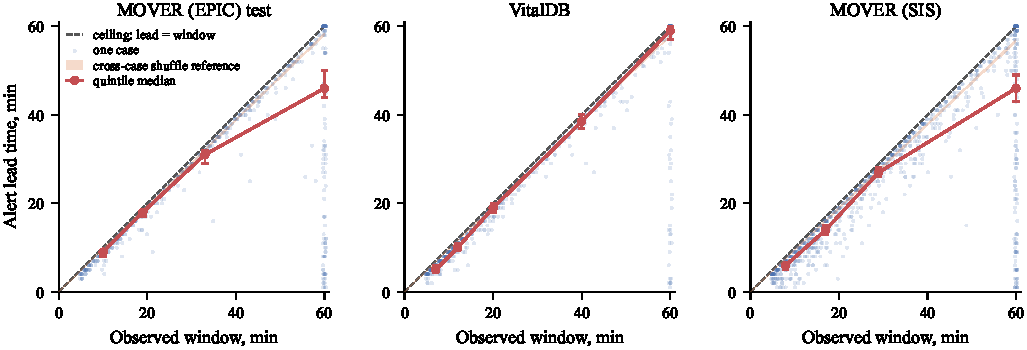
\includegraphics[width=\linewidth]{figures/Figure_2_wide.pdf}
  \caption{\textbf{Alert lead time against the available pre-onset window.} Every detected event case under the ITE Transformer, three held-out cohorts. The dashed diagonal is the ceiling: no crossing can be found outside the case's own window. The shaded band is the 2.5th to 97.5th percentile envelope of the cross-case shuffle reference, not a per-case prediction interval. Red markers are the band medians of Table A9 with 95\% cluster bootstrap intervals; all five families are Figure A1.}
  \label{fig:1}
\end{figure}

\subsection{Explicit references for the ceiling dependence}\label{explicit-references-for-the-ceiling-dependence}

Part of the relationship is built into the definition: a lead time cannot exceed the window it is
searched in, so the ratio is bounded in {[}0, 1{]} by construction and positive dependence can arise
without patient-specific timing. A bound does not specify a distribution, so we use two explicit
references rather than treating the diagonal as a null.

\textbf{The interpretive rule comes before the numbers, because it decides what they can mean.} Both
references are biased \emph{toward} agreement with the observed values, in the direction that favors our
own reading, so each is an upper bound on what a window-only process could produce. A reference
that reaches or exceeds the observed value is therefore the expected and uninformative outcome;
what would be informative is one falling clearly short, and neither does.

\textbf{A continuous uniform reference has median 0.5.} Placing a pseudo-crossing uniformly on each
case's own window gives a reference median of 0.518 to 0.534, which the observed ratio exceeds by
\textbf{+0.372 to +0.421} for the transformer. It does not exceed it everywhere: in \textbf{2 of 15} cells
the observed ratio sits \emph{below} the reference and in one more it is indistinguishable from it, all
three VitalDB cells (Table A2).

\textbf{A cross-case shuffle preserves the aggregate relationship} (Figure 1). Each recipient keeps its
window and reference time but receives another case's whole score sequence, aligned by elapsed
window time, so generic elapsed-time shape survives while the match between trajectory and
recipient is destroyed. Permutations are derangements, 1,000 per cell, so no case keeps its own
sequence. The shuffled median ratio is \textbf{0.72 to 0.97} and
Spearman \textbf{0.63 to 0.94}, so the reference exceeds the observed ratio in \textbf{15 of 15} cells,
which under the rule above is what an upward-biased reference is expected to do. Under a
length-matched variant the observed correlation is \textbf{not distinguishable from the reference in 9
of 15 cells}, and the reference is the larger in 6 of 15 (Table A2).

\textbf{Under these deliberately conservative references the observed association did not exceed what a
window-only reassignment can produce.} That is not the same as showing that a window-only process
generates it, nor that patient-specific information is absent. Reassignment also changes which
event cases are detected, and both variants bias upward, by selecting longer, already-settled
donors or holding a short donor's last value. They bound the dependence rather than estimating a
case-independent process.

\section{Score behavior behind the reported lead}\label{score-behavior-behind-the-reported-lead}

Section 4.1 identifies a direct mechanism for one model. A cross-family property of the score
paths is consistent with it without establishing its cause, and is reported in Appendix A.4
beside Table A3.

\subsection{The transformer is above its own alert threshold almost immediately, in event and control alike}\label{the-transformer-is-above-its-own-alert-threshold-almost-immediately-in-event-and-control-alike}

This section asks what the score is doing at the minutes the alert rule reads, and what the
operating point behind the reported lead looks like.

\textbf{Within one minute of its first scored minute the transformer's median score is already
above the threshold its operating point uses, and it is there for event and control cases
equally} (Figure A5).

In MOVER (EPIC) the median score rises from 0.530 at the first scored minute to 0.938 one
minute later in control cases, and from 0.541 to 0.951 in event cases, against a transported
threshold of \textbf{0.894}. By minute five the two groups are at 0.973 and 0.975, a separation of
0.002 in a score whose scale runs to 1. VitalDB behaves the same way, reaching 0.966 and
0.973. MOVER (SIS) settles more slowly, at 0.833 and 0.906 by minute two and 0.942 and 0.962
by minute five, but it too clears the threshold and it too does so in both groups.

The consequence for the metric is direct. A case whose score settles above the threshold
within its first monitored minutes will register its first crossing as soon as its alert
window opens, whatever else happens, so its lead time is whatever that window holds. That is
the near one-for-one contrast in Table A9.

\textbf{No other family does this} (Figure A5). Sustained elevation is visible in the share of
monitored minutes at or above threshold: \textbf{20.0 to 52.3\% of the transformer's event minutes and
2.5 to 18.3\% of its control minutes, against 0 to 26.7\% and 0 to 1.7\% for the other four
families}.

\textbf{The obvious objection is that this model simply alerts continuously, and reporting the
operating point beside the lead shows that it largely does} (Table 1). Its case-level
specificity is 0.406, 0.379 and 0.467, so it alerts on 53 to 62\% of control cases, and its
positive predictive value of 0.625, 0.380 and 0.585 sits 0.065, 0.021 and 0.051 above the
prevalence it is measured against. This is not a competing explanation of Section 3 but the same
fact: a score above threshold most of the time alerts at the first opportunity, which is what
makes the lead the window. The point is that \textbf{the reported lead carries none of it.} A median
lead of 24, 17 and 22 minutes is the largest of the fifteen combinations and comes from the one
with the least usable operating point.

That holds beyond one model. \textbf{Across the fifteen combinations the reported median lead runs
opposite to case-level specificity} (Spearman $-$0.803, permutation \emph{P} = 0.0008, \emph{q} = 0.006; 86
of 99 untied pairs), and opposite to PPV in excess of prevalence at $-$0.719. Within a cohort the
ordering is 9 of 9 untied pairs in both MOVER cohorts and 8 of 10 in VitalDB, but five
combinations per cohort is thin and none survives adjustment alone, so the pooled figure carries
the claim and cohort confounds it. Two further limits belong with it. The unit is a combination
and not a patient, so these are permutations of the pairing rather than cluster bootstraps. And a
transported threshold does not deliver the same realized sensitivity everywhere: it runs from
0.461 to 0.849 across these combinations (Table A4), so this is a descriptive association among
the operating points as transported, not a sensitivity-matched ranking of models. What it
supports is narrower and still worth stating: a reader ranking these systems by the number they
publish would not be ranking them by how usable their operating points are.

\textbf{Table 1 \textbar{} Case-level operating point behind each reported lead time.} ITE Transformer, three
held-out cohorts, at the transported 80\%-sensitivity operating point every lead time in this paper
uses. \texttt{Min.\ above\ thr.} is the median share of an event case's monitored minutes at or above
threshold. Event prevalence is a property of the cohort, not the cell: 0.560, 0.359 and 0.534.
\textbf{All five families, every interval, the number needed to evaluate, the control-side burden and PPV
in excess of prevalence are Table A4}, where the cross-family claim below is checked.

\begin{longtable}[]{@{}llrrrrr@{}}
\toprule
Model & Cohort & Sens. & Spec. & PPV & Min. above thr. & Lead, min \\
\midrule
\endhead
Transformer & EPIC test & 0.777 & 0.406 & 0.625 & 0.523 & 24 \\
Transformer & VitalDB & 0.679 & 0.379 & 0.380 & 0.444 & 17 \\
Transformer & MOVER SIS & 0.657 & 0.467 & 0.585 & 0.200 & 22 \\
\bottomrule
\end{longtable}

\subsection{What these findings do and do not license}\label{what-these-findings-do-and-do-not-license}

Both findings are properties of a pipeline as deployed with this scoring policy rather than claims
about what any architecture must do; Section 7 states the scope. Neither is a claim about
physiology. The outcome is a sustained excursion of mean arterial pressure and mean arterial
pressure is one of the model's input channels, so the model has direct access to the quantity the
label is computed from, and nothing here shows that a score anticipates a physiological process.

\section{Two natural remedies, and why neither works}\label{two-natural-remedies-and-why-neither-works}

Two fixes follow naturally from Sections 3 and 4, and neither works. A metric with a
plausible-looking repair that fails is a worse problem than one with none, because the repair
gets adopted.

\subsection{Prevalent alerts are not the explanation}\label{prevalent-alerts-are-not-the-explanation}

The first thought is that the metric is dominated by cases already above threshold at their first
eligible minute. Such cases are
\textbf{2.6 to 25.5\%} of detected event cases across
the fifteen cells, and removing them to recompute the median lead on incident alerts alone costs
\textbf{0 to 3 minutes in all fifteen cells}, the transformer included (Appendix A.11).
The relationship of Section 3 is therefore carried by the ordinary cases. Prevalence stays this low
alongside the settling of Section 4.1 because most detected event cases have an available window
shorter than 60 minutes, so it opens while the score is still settling: prevalence and a warm-up
crossing are the same behavior on either side of that minute.

\subsection{Suppressing the first minutes of monitoring is not the fix}\label{suppressing-the-first-minutes-of-monitoring-is-not-the-fix}

The second thought follows from Section 4.1: if the score is unreliable while it settles, discard
alerts raised during that period. We implemented exactly that, discarding every minute at or before
\emph{N} minutes of elapsed monitoring and then applying the unchanged threshold.

At \emph{N} = 5, across all five families and three cohorts, the rule costs \textbf{3.6 to 6.8
percentage points of case-level sensitivity} and returns \textbf{0 to 3.2 percentage points of
specificity}. Median lead changes by \textbf{$-$3 to +1 minutes}; in two of the fifteen cells it
\emph{increases}, because discarding early minutes removes some short-window cases from the detected
set entirely and shifts the median. The trade is poor in every cell, and it does not address
Section 3: the surviving alerts still fire at the first opportunity within whatever window
remains.

The comparison holds the transported threshold fixed, so it is deliberately unmatched on
sensitivity; reselecting a threshold is the one thing this paper does nowhere. The direction is not
expected to reverse under matching: suppression removes alerting minutes and cannot add crossings,
so after lowering the threshold to restore sensitivity, any specificity gain cannot exceed the
fixed-threshold gain above.

\textbf{We therefore do not recommend the rule.} The problem is not that early minutes are noisy.
It is that the reported quantity is coupled to the length of the window it was measured in.

\subsection{What partially helps, and what remains}\label{what-partially-helps-and-what-remains}

Both repairs above change the alert rule and leave the estimand alone. The remaining option
reverses that: condition on window length, or treat the first alert as a time-to-event whose
follow-up ends when the window does, the landmarking treatment of a prediction made at a fixed
point in a run-up \citep{vanhouwelingen2007landmark}. Both are computable from the same cached scores,
so we report them rather than only recommending them (Tables A6 and A7).

\textbf{A horizon-specific detection rate reduces the dependence rather than removing it.} It makes the
horizon explicit and conditions the denominator on event cases observed for at least \emph{X} minutes
before onset. That removes one ambiguity of the pooled median, but window length is still not
constant: cases observed longer than \emph{X} can contribute different amounts of pre-horizon alerting
opportunity. The rate runs 0.278 to 0.692 at a 10-minute horizon and 0.173 to 0.547 at 30 minutes,
declining smoothly with the horizon, a shape a single median suppresses (Table A6).
Restricted instead to cases observed for the whole 60-minute window, so the window is a constant,
the transformer reports the longest median lead of the five families in all three cohorts, 47, 60
and 57 minutes, while detecting only 0.441, 0.247 and 0.304 of them against 0.762 to 0.910 for
XGBoost and the random forest (Table A7): conditioning turns its reported advantage into a deficit.

\textbf{Both remain partial.} The full-window restriction is the stricter window-constant estimand, but
it changes the estimand and the population, discarding 53 to 60\% of event cases: the short-window
cases a deployed monitor will meet. The horizon-specific curve keeps more cases at short horizons
but does not equalize pre-horizon alerting opportunity. Neither repairs the pooled headline median,
and for the reason given in Section 2 the censoring is not independent of the event, with short-
and long-run-up cases differing in surgery duration and case mix (Appendix A.12).

\section{A task-specific reporting extension}\label{a-task-specific-reporting-extension}

Reporting conventions decide what interpretation is available to a reader. A clinician,
policymaker or science writer meets a number and a name, not the scoring policy behind them, so
what a standard asks for bounds what any of them can conclude. That is why auditing one metric is
a communication result and not only a metrology one.

\textbf{This section maps that case study onto what a general standard explicitly asks for.} A
TRIPOD+AI checklist was completed for this work by its own authors, before Sections 3 to 5 were
conducted, and it did not request the disclosures that reveal the dependence. TRIPOD+AI is a
general minimum \textbf{reporting} standard rather than a validity tool, and one author-completed
checklist cannot assess a general framework in either direction. So what follows is a mapping,
and the items in Section 6.2 are task-specific candidate disclosures that complement the standard
rather than correct, invalidate or demonstrate non-adherence to it.

\subsection{The items that were satisfied}\label{the-items-that-were-satisfied}

\textbf{Item 12e, performance measures and rationale}, is where a lead time is declared: it asks
\emph{which} measures were used and \emph{why}, not what else a measure could be responding to. \textbf{Item 23a,
model performance}, asks for performance with uncertainty, and Table 1 satisfies it. So Table 1
is a compliant table in which a 24-minute lead sits beside a specificity of 0.406, with nothing in
either item requiring a reader to put the two together. Four further items came close and missed
(Table A8), and one pattern runs across them: the available pre-onset window distribution is never
requested, and it is the variable the reported lead correlates with at $\rho$ = 0.501 to 0.906.

\textbf{Item 14, model fairness, is the near miss}, and the most instructive item on the list. The
checklist's own fairness answer records that arterial-line placement selects toward longer,
higher-risk operations. The information that observation length is not distributed at random was
therefore \textbf{already disclosed}, filed as a limitation, where it reads as a caveat about which
patients the findings extend to. Nothing in the standard connects it to the timing metric three
tables away.

\subsection{Four candidate disclosures for continuously monitored models}\label{four-candidate-disclosures-for-continuously-monitored-models}

Each is tied to a measurement in this paper, each is computable from artifacts a study of this
kind already produces, and none requires a new experiment. They have not been validated as a
general reporting framework.

\begin{enumerate}
\def\labelenumi{\arabic{enumi}.}
\item
  \textbf{Report alert composition by elapsed observation time}: for every operating point, the share
  of alerts already active at the first eligible minute, those that fired within a short settling
  period, and those that fired later (Figure A2). One stacked bar would have made Section 4.1
  visible on inspection.
\item
  \textbf{Report a window-conditional timing statistic as the primary timing quantity.} A
  horizon-specific detection curve may be added as a secondary disclosure, provided its
  denominator and its remaining dependence on pre-horizon alerting opportunity are stated. Any
  single median should be secondary and stratified by the distribution of available pre-onset
  windows it was measured over: the transformer reports 5 to 9 minutes for its shortest-window
  band and 46 to 59 for its longest, and the pooled 17 to 24 carries neither. Tables A6 and A7
  show the two alternatives; Section 5.3 gives their limits.
\item
  \textbf{Report N(t) beside any event-aligned trajectory.} Here the risk set roughly halves between
  the event and 60 minutes before it (1,404 to 708, 2,804 to 1,433 and 2,641 to 1,374), and the
  cases surviving to the far end are the long-window ones, the same selection that drives
  Section 3. \textbf{The denominator is not cosmetic}: recomputing the same bins on only the cases
  observable back to 60 minutes moves the first bin reaching AUROC 0.70 from 15 minutes in all
  three cohorts to 20, 35 and 20, so the horizon a reader would quote changes by up to twenty
  minutes on a reporting choice alone, and neither curve is the true one (Figure A3).
\item
  \textbf{Report a path-versus-displacement summary for any score read as a trend}, so that a series
  travelling much farther than its net displacement is qualified before it is described as rising
  or falling (Table A3 and Appendix A.4).
\end{enumerate}

The first three are disclosure items in the ordinary TRIPOD sense, naming a quantity that must
appear beside one already required; the fourth is closer to a diagnostic, and we offer it as the
weakest of the four for that reason.

\subsection{What this does and does not generalize to}\label{what-this-does-and-does-not-generalize-to}

The specific artifact does not generalize; its shape does. The shape is a quantity named for what
a clinician would experience,
computed from a window whose length varies across patients and is not reported, under a standard
that requires the quantity and not the window. Any continuously read model evaluated with a
first-crossing statistic over variable available windows is structurally susceptible to this
dependence. Its empirical magnitude has to be measured in each setting, and the four items are the
disclosure that would let a reader see it.

\section{Limitations and scope}\label{limitations-and-scope}

\textbf{Retrospective, and one label.} Every score is computed from cached data after the fact: a
retrospective forward-running simulation, not deployment clearance. The outcome is a sustained
excursion of mean arterial pressure below a fixed level, and both the level and the duration are
conventions we did not vary; the label's dependence on a channel the models read is in Section 4.2.

\textbf{One model fit, one family of operating points, and one draw of the control reference times.}
Models were trained at one seed and thresholds come from one validation split at one sensitivity
target, transported unchanged; a different fit or target could move the composition of Section 5.1,
the magnitudes of Section 3 and the operating points of Table 1, and we varied none of them.
Control cases have no onset, so each is assigned a pseudo-onset sampled once at a fixed seed from
the event cases' timing distribution. \textbf{Every control-side quantity here is conditional on that
one draw}: the case-level specificity and positive predictive value of Table 1, the control-side
minute share, and the cross-combination association of Section 4.1 that rests on them. Its
resampling variability is not propagated into any interval we report. Redrawing the reference
times would require rerunning the complete control-side evaluation pipeline for every model and
cohort, so we report all control-side quantities as conditional on the single pre-specified draw
rather than presenting an unperformed sensitivity analysis.

\textbf{Properties of a pipeline, not of an architecture.} Section 4.1 describes what one model does
under one scoring policy on these cohorts, not what sequence models must do. Section 3's effect is
present in all five families, the ratio running 0.455 to 0.944, with the transformer the limiting
case rather than the exception.

\textbf{The references bias upward.} Both shuffle variants make agreement easier to obtain, in the
direction that favors our own reading, and they change the detected-case set. They bound the
dependence rather than estimating a case-independent process.

\textbf{Communication and reporting claims, and one clinical domain.} We analyze the interpretation
invited by the metric's name, not measured clinician comprehension. The TRIPOD+AI assessment was
author-completed, and the four disclosures were demonstrated here rather than validated across
reporting settings or stakeholder groups. Three cohorts, two health systems and two countries
still give one procedure setting and one monitored variable, so they cannot settle whether
Section 6.2's four items are the right four elsewhere.



% References start on their own page. Without this they begin wherever the body happens to
% end, which under Tectonic is page 9 only because the body fills page 8 to the bottom --
% pdfLaTeX on Overleaf breaks lines slightly differently, leaves room on page 8, and starts
% the reference list directly under the Conclusion. \appendix and the checklist already
% \clearpage; this was the one unguarded boundary, so the page map now holds on any engine.
\clearpage

\bibliographystyle{plainnat}
% latex/references.bib is COPIED here by build_tex.py from ../references.bib on
% every run, and is gitignored. Do not edit it: edit ../references.bib.
% BibTeX will not follow a \bibliography{../references} path reliably -- that
% silently produced an empty reference list -- so a synced copy is the fix, not
% a relative path.
\bibliography{references}

% appendix.tex opens with its own \clearpage, so the appendix starts on a fresh page after
% the references. It also sets \appendix, \raggedbottom and the A-numbering for sections
% and figures; see build_tex.py for why each is needed.
\clearpage
\appendix
\raggedbottom
\renewcommand{\thesection}{Appendix \Alph{section}}
\renewcommand{\thesubsection}{\Alph{section}.\arabic{subsection}}
\setcounter{figure}{0}
\renewcommand{\thefigure}{A\arabic{figure}}
\renewcommand{\theHfigure}{A\arabic{figure}}
\section{Methods and complete per-cell results}

\subsection{Cohorts, models, training and compute}\label{cohorts-models-training-and-compute}

\textbf{Cohorts and eligibility.} Two public datasets supply the three cohorts: VitalDB, and
MOVER, whose single release carries both an EPIC-derived and an SIS-derived arm. Both are de-identified. VitalDB v1.0.0 is openly accessible from PhysioNet under the Creative Commons Attribution 4.0 International (CC BY 4.0) license; MOVER is available from the UCI Machine Learning Repository to researchers who sign its data use agreement. Development
used MOVER's EPIC arm. The subject-aware split at
seed 1004 gave 6,409 training, 1,375 validation and 1,404 test cases
out of 9,188, split on unique subject identifiers so that a patient with several operations
lands in one fold. The test split holds 1,404 cases, 786 with a sustained event, 1,145 subjects.
External evaluation used VitalDB, with 2,804 cases, 1,007 events and 2,730 subjects, and the
SIS-derived arm of MOVER, with 2,641 cases and 1,409 events, neither of which contributed to training, calibration or threshold selection. Neither arm of MOVER carries a subject key that resolves against the other, so that statement holds at the level of the released records and cannot be checked at the level of patients. Per-minute eligibility
drops the induction prefix, 25 minutes where the record is anchored on anesthesia start, 10
where it is anchored on surgical start, and every minute at or after first onset, so no
model is asked to predict an event already in progress. Event cases required five valid
pre-onset minutes after that exclusion and controls thirty. Procedure group is never a model
input in any family: it separates the cohorts almost perfectly and would be learned as cohort
identity.

\textbf{Training samples, labels and the offset used here.} Training uses one sample per case: the
120-minute window ending at that case's reference time, labeled 1 if the case has a sustained
event and 0 otherwise. There is no per-minute training target. For an event case the reference
time is the first sustained-onset minute shifted back by a lead-time offset, and that offset is
\textbf{zero for every model reported in this paper}, so the reference time is onset itself. A control
has no onset, so it is given a sampled pseudo-onset: its onset ratio, onset divided by case
length, is drawn with replacement from the event cases of the same source cohort and multiplied
by the control's own case length, then resampled rather than clipped until it falls inside the
eligible range, so the control reference times match the event distribution within each source.
Event cases with fewer than five eligible pre-onset minutes and controls shorter than thirty are
dropped before that sampling. The scored checkpoint is the epoch with the best validation AUROC,
and it is the only one used. Evaluation departs from training in the one respect that matters
here: every eligible minute of a case is scored independently and inherits its case's label, and
\texttt{t\_\allowbreak{}to\_\allowbreak{}event} is measured against that same reference time, real onset for an event case and the
sampled pseudo-onset for a control.

\textbf{Features.} The same twenty inputs for every family: sixteen per-minute channels, being
MAP, systolic and diastolic pressure, their non-invasive counterparts, heart rate, SpO2,
end-tidal CO2, temperature, FiO2, MAC, tidal volume, respiratory rate, PEEP and peak
inspiratory pressure, and four demographics, being age, sex, height and weight. The families
differ in how they consume them. The transformer takes each non-missing cell as a
(type, time, value) triplet with demographics as a fixed prefix at time zero, up to 2,048
tokens over a 120-minute window, so missing cells produce no token and are never imputed. The
LSTM takes the normalized per-minute window as a value-and-mask pair per channel. Logistic
regression, random forest and XGBoost take the last observation carried forward per channel
plus the demographics. Per-channel median and interquartile scaling was fitted on the
training cases alone and applied unchanged everywhere else.

\textbf{Architectures and training.} Seed 1004 throughout. The transformer is a STraTS-style
encoder, a type embedding plus a value MLP plus a time MLP summed per triplet, two encoder
layers, model width 128, four heads, feed-forward width 512, dropout 0.1, a learnable
classification token and a two-class softmax head; AdamW at learning rate 1.2e-3, weight
decay 1e-2 applied to two-dimensional tensors only, gradient clipping at 1.0, a cosine
schedule with 5\% warmup, batch size 64, cross-entropy, up to 50 epochs with early stopping on
validation AUROC at patience 10, under bfloat16 autocast. The LSTM is one layer of width 128
with dropout 0.1, AdamW at 1e-3 with weight decay 1e-2, batch size 64, up to 40 epochs at
patience 8. Logistic regression is median imputation and standardization followed by an L2
fit at up to 2,000 iterations. The random forest is 400 trees. XGBoost is 600 rounds at depth
6, learning rate 0.05, row and column subsampling at 0.8, histogram tree method, early
stopping after 40 rounds on validation AUC. No hyperparameter search was run over any of
these values.

\textbf{Compute.} Every model was trained on one Apple M3 Ultra desktop with 512 GB of unified
memory, using PyTorch 2.10 on the Metal backend with bfloat16 autocast; no GPU cluster was
used. Wall clock for the five models reported here was 40.3 minutes for the transformer, 14.5
for the LSTM, 3.6 for the random forest, and 34 and 33 seconds for XGBoost and logistic
regression. The project trained more than this paper reports: each family was also trained at
seven lead-time offsets, of which the transformer arm alone took 3.8 hours. The analyses in
this paper add no training and read cached per-minute scores on the same machine. Software
was PyTorch 2.10.0, scikit-learn 1.7.1, XGBoost 3.3.0, NumPy
2.2.6, pandas 2.3.2 and SciPy 1.16.1.

\textbf{Data and code.} Both source datasets are public and de-identified. VitalDB v1.0.0 is openly accessible from PhysioNet under the Creative Commons Attribution 4.0 International (CC BY 4.0) license; MOVER is available from the UCI Machine Learning Repository under its data use agreement, one download supplying both arms used here. An
institutional review board granted this secondary analysis an exemption from review and a
waiver of consent, its identity and protocol number withheld for anonymous review. This work
added no data collection and no patient contact. Analysis code is available at an anonymized repository,
\url{https://anonymous.4open.science/r/ioh-leadtime-anon-BD0E}, under the Apache License 2.0.
The repository carries the analysis code and the aggregate result files behind the tables and figures, and no patient-level or derived patient-level data of any kind; each dataset is obtained from its own provider under the access and license terms above.

\subsection{Lead time by quantile-derived band of observed window, all fifteen cells}\label{lead-time-by-quantile-derived-band-of-observed-window-all-fifteen-cells}

\begin{minipage}{\linewidth}
\textbf{Table A1 \textbar{} Median alert lead time by quantile-derived band of observed window, all fifteen
cells.} Main text Section 3.1 reports the ITE Transformer. The gradient is positive in
every cell.
\texttt{Bands} is the number of quantile-derived groups actually realized: where the observed window is censored
at the 60-minute alert window the upper quintiles collapse onto a single value, and
duplicate edges are dropped rather than bands invented.
The gradient is the difference of the highest and lowest band medians, and its interval is the
paired cluster bootstrap of that difference: one weight matrix is drawn per cell and reused
across bands, and the band edges and the window span are held fixed at their full-sample values
so the ratio's denominator is not itself resampled. The interval excludes zero in all fifteen
cells. \texttt{Lead\ min\ per\ window\ min} is the ratio of those two between-band median contrasts and not
a per-case slope, so a value slightly above 1.0 carries no contradiction with the per-case
constraint that a lead cannot exceed its own window.

\vspace{0.5em}
\centering\footnotesize
\begin{tabular}{@{}
  >{\raggedright\arraybackslash}p{(\columnwidth - 12\tabcolsep) * \real{0.14}}
  >{\raggedright\arraybackslash}p{(\columnwidth - 12\tabcolsep) * \real{0.14}}
  >{\raggedleft\arraybackslash}p{(\columnwidth - 12\tabcolsep) * \real{0.18}}
  >{\raggedright\arraybackslash}p{(\columnwidth - 12\tabcolsep) * \real{0.14}}
  >{\raggedright\arraybackslash}p{(\columnwidth - 12\tabcolsep) * \real{0.14}}
  >{\raggedright\arraybackslash}p{(\columnwidth - 12\tabcolsep) * \real{0.14}}
  >{\raggedright\arraybackslash}p{(\columnwidth - 12\tabcolsep) * \real{0.14}}@{}}
\toprule
Model & Cohort & Bands & Window Q1$\rightarrow$last, min & Lead Q1$\rightarrow$last, min & Gradient, min (95\% CI) & Lead min per window min (95\% CI) \\
\midrule
Transformer & MOVER (EPIC) test & 4 & 10 $\rightarrow$ 60 & 9 $\rightarrow$ 46 & +37 {[}+35, +41{]} & 0.74 {[}0.70, 0.82{]} \\
Transformer & VitalDB & 5 & 7 $\rightarrow$ 60 & 5 $\rightarrow$ 59 & +54 {[}+51, +55{]} & 1.02 {[}0.96, 1.04{]} \\
Transformer & MOVER (SIS) & 4 & 8 $\rightarrow$ 60 & 6 $\rightarrow$ 46 & +40 {[}+37, +43{]} & 0.77 {[}0.71, 0.83{]} \\
LSTM & MOVER (EPIC) test & 4 & 10 $\rightarrow$ 60 & 6 $\rightarrow$ 44 & +38 {[}+35, +41{]} & 0.77 {[}0.70, 0.82{]} \\
LSTM & VitalDB & 5 & 6 $\rightarrow$ 60 & 3 $\rightarrow$ 34 & +31 {[}+21, +48{]} & 0.57 {[}0.39, 0.89{]} \\
LSTM & MOVER (SIS) & 4 & 9 $\rightarrow$ 60 & 5 $\rightarrow$ 31 & +26 {[}+19, +30{]} & 0.51 {[}0.37, 0.59{]} \\
XGBoost & MOVER (EPIC) test & 3 & 12 $\rightarrow$ 60 & 8 $\rightarrow$ 38 & +30 {[}+26, +34{]} & 0.62 {[}0.54, 0.71{]} \\
XGBoost & VitalDB & 3 & 9 $\rightarrow$ 60 & 3 $\rightarrow$ 30 & +27 {[}+22, +30{]} & 0.53 {[}0.43, 0.58{]} \\
XGBoost & MOVER (SIS) & 3 & 12 $\rightarrow$ 60 & 5 $\rightarrow$ 36 & +31 {[}+28, +33{]} & 0.65 {[}0.58, 0.69{]} \\
Random forest & MOVER (EPIC) test & 3 & 13 $\rightarrow$ 60 & 8 $\rightarrow$ 38 & +30 {[}+26, +34{]} & 0.64 {[}0.55, 0.72{]} \\
Random forest & VitalDB & 3 & 9 $\rightarrow$ 60 & 3 $\rightarrow$ 34 & +31 {[}+29, +34{]} & 0.61 {[}0.57, 0.67{]} \\
Random forest & MOVER (SIS) & 3 & 12 $\rightarrow$ 60 & 6 $\rightarrow$ 40 & +34 {[}+31, +36{]} & 0.71 {[}0.65, 0.75{]} \\
Logistic reg. & MOVER (EPIC) test & 3 & 11 $\rightarrow$ 60 & 8 $\rightarrow$ 40 & +32 {[}+28, +35{]} & 0.65 {[}0.57, 0.71{]} \\
Logistic reg. & VitalDB & 3 & 10 $\rightarrow$ 60 & 3 $\rightarrow$ 28 & +26 {[}+20, +28{]} & 0.51 {[}0.40, 0.56{]} \\
Logistic reg. & MOVER (SIS) & 3 & 12 $\rightarrow$ 60 & 5 $\rightarrow$ 38 & +33 {[}+29, +36{]} & 0.69 {[}0.61, 0.75{]} \\
\bottomrule
\end{tabular}
\end{minipage}

\vspace{0.8em}

\subsection{Both nulls, all fifteen cells}\label{both-nulls-all-fifteen-cells}

\begin{minipage}{\linewidth}
\textbf{Table A2 \textbar{} Both nulls, all fifteen cells.} Observed ratio against the
uniform-placement null of Section 3.3 and both variants of the
cross-case shuffle. The uniform null's expectation is 0.5 by construction; the two shuffle
variants differ only in how a donor shorter than its recipient is handled, and both bias
the null upward. Intervals are the 2.5th and 97.5th percentiles of the null distribution.

\vspace{0.5em}
\centering\footnotesize
\begin{tabular}{@{}
  >{\raggedright\arraybackslash}p{(\columnwidth - 16\tabcolsep) * \real{0.130}}
  >{\raggedright\arraybackslash}p{(\columnwidth - 16\tabcolsep) * \real{0.100}}
  >{\raggedleft\arraybackslash}p{(\columnwidth - 16\tabcolsep) * \real{0.125}}
  >{\raggedright\arraybackslash}p{(\columnwidth - 16\tabcolsep) * \real{0.100}}
  >{\raggedright\arraybackslash}p{(\columnwidth - 16\tabcolsep) * \real{0.100}}
  >{\raggedright\arraybackslash}p{(\columnwidth - 16\tabcolsep) * \real{0.100}}
  >{\raggedleft\arraybackslash}p{(\columnwidth - 16\tabcolsep) * \real{0.125}}
  >{\raggedright\arraybackslash}p{(\columnwidth - 16\tabcolsep) * \real{0.100}}
  >{\raggedright\arraybackslash}p{(\columnwidth - 16\tabcolsep) * \real{0.100}}@{}}
\toprule
Model & Cohort & Observed ratio & Uniform null & Shuffle null, hold & Shuffle null, length-matched & Observed $\rho$ & Shuffle $\rho$, hold & Shuffle $\rho$, length-matched \\
\midrule
Transformer & MOVER (EPIC) test & 0.944 & 0.524 {[}0.491, 0.567{]} & 0.970 {[}0.967, 0.974{]} & 0.962 {[}0.951, 0.971{]} & 0.706 & 0.888 {[}0.855, 0.920{]} & 0.783 {[}0.705, 0.856{]} \\
Transformer & VitalDB & 0.923 & 0.532 {[}0.500, 0.573{]} & 0.966 {[}0.963, 0.967{]} & 0.957 {[}0.947, 0.969{]} & 0.906 & 0.941 {[}0.926, 0.955{]} & 0.933 {[}0.890, 0.967{]} \\
Transformer & MOVER (SIS) & 0.899 & 0.527 {[}0.500, 0.567{]} & 0.949 {[}0.941, 0.950{]} & 0.918 {[}0.900, 0.938{]} & 0.801 & 0.877 {[}0.855, 0.895{]} & 0.775 {[}0.713, 0.827{]} \\
LSTM & MOVER (EPIC) test & 0.851 & 0.522 {[}0.483, 0.563{]} & 0.913 {[}0.900, 0.923{]} & 0.866 {[}0.833, 0.893{]} & 0.650 & 0.825 {[}0.784, 0.860{]} & 0.673 {[}0.596, 0.743{]} \\
LSTM & VitalDB & 0.619 & 0.534 {[}0.500, 0.583{]} & 0.870 {[}0.850, 0.883{]} & 0.752 {[}0.667, 0.833{]} & 0.759 & 0.845 {[}0.798, 0.886{]} & 0.705 {[}0.593, 0.804{]} \\
LSTM & MOVER (SIS) & 0.717 & 0.524 {[}0.500, 0.562{]} & 0.873 {[}0.857, 0.887{]} & 0.700 {[}0.633, 0.767{]} & 0.501 & 0.682 {[}0.636, 0.727{]} & 0.455 {[}0.368, 0.547{]} \\
XGBoost & MOVER (EPIC) test & 0.719 & 0.519 {[}0.483, 0.558{]} & 0.842 {[}0.814, 0.867{]} & 0.760 {[}0.705, 0.800{]} & 0.558 & 0.701 {[}0.651, 0.751{]} & 0.581 {[}0.503, 0.649{]} \\
XGBoost & VitalDB & 0.467 & 0.521 {[}0.483, 0.556{]} & 0.723 {[}0.667, 0.768{]} & 0.591 {[}0.517, 0.652{]} & 0.599 & 0.636 {[}0.569, 0.698{]} & 0.493 {[}0.400, 0.580{]} \\
XGBoost & MOVER (SIS) & 0.600 & 0.518 {[}0.500, 0.550{]} & 0.779 {[}0.750, 0.800{]} & 0.681 {[}0.633, 0.722{]} & 0.573 & 0.632 {[}0.590, 0.673{]} & 0.488 {[}0.429, 0.541{]} \\
Random forest & MOVER (EPIC) test & 0.714 & 0.519 {[}0.483, 0.556{]} & 0.839 {[}0.816, 0.867{]} & 0.777 {[}0.733, 0.817{]} & 0.584 & 0.714 {[}0.665, 0.764{]} & 0.599 {[}0.531, 0.667{]} \\
Random forest & VitalDB & 0.533 & 0.523 {[}0.500, 0.556{]} & 0.764 {[}0.721, 0.800{]} & 0.685 {[}0.625, 0.733{]} & 0.651 & 0.678 {[}0.622, 0.729{]} & 0.555 {[}0.479, 0.627{]} \\
Random forest & MOVER (SIS) & 0.667 & 0.518 {[}0.500, 0.550{]} & 0.811 {[}0.783, 0.833{]} & 0.741 {[}0.700, 0.783{]} & 0.618 & 0.659 {[}0.625, 0.692{]} & 0.536 {[}0.486, 0.589{]} \\
Logistic reg. & MOVER (EPIC) test & 0.781 & 0.520 {[}0.483, 0.557{]} & 0.872 {[}0.849, 0.898{]} & 0.802 {[}0.767, 0.842{]} & 0.597 & 0.739 {[}0.694, 0.779{]} & 0.612 {[}0.544, 0.676{]} \\
Logistic reg. & VitalDB & 0.455 & 0.521 {[}0.471, 0.567{]} & 0.721 {[}0.667, 0.781{]} & 0.577 {[}0.500, 0.650{]} & 0.607 & 0.642 {[}0.549, 0.720{]} & 0.486 {[}0.374, 0.584{]} \\
Logistic reg. & MOVER (SIS) & 0.618 & 0.518 {[}0.500, 0.550{]} & 0.782 {[}0.750, 0.800{]} & 0.734 {[}0.692, 0.767{]} & 0.597 & 0.644 {[}0.607, 0.682{]} & 0.548 {[}0.495, 0.595{]} \\
\bottomrule
\end{tabular}
\end{minipage}

\vspace{0.8em}

Three cells in this table are the ones Section 3.3 names as not exceeding the uniform
reference, all of them VitalDB. The observed ratio sits below it for XGBoost by $-$0.054 and for
logistic regression by $-$0.067, and random forest is indistinguishable from it (+0.011,
\emph{P} = 0.824). For the transformer the excess over the uniform reference is +0.372 to +0.421.
Under the length-matched shuffle variant the transformer's null spans 0.77 to 0.93. Every
contrast quoted here is computed from the unrounded values rather than from the rounded columns
above, so recomputing one from the table can differ in the third decimal.

\subsection{Path decomposition}\label{path-decomposition}

\begin{minipage}{\linewidth}
\textbf{Table A3 \textbar{} Path decomposition over the window 60 to 5 minutes before onset.} Event
episodes have observed scores at both window edges. Directedness
is net displacement divided by total distance traveled, so 1 is a monotone climb and 0 is a
round trip. Path per net is total distance divided by the absolute net change. Episodes
observed at every bin center in the window; median 11 steps per episode. Intervals are 95\%
cluster bootstrap. Only this window is reported: over 60 to 10 minutes the transformer's net
displacement is indistinguishable from zero in two cohorts, and the ratio is then a division
by approximately nothing.

\vspace{0.5em}
\centering\footnotesize
\begin{tabular}{@{}llrlr@{}}
\toprule
Cohort & Model & Episodes & Directedness (95\% CI) & Path per unit net \\
\midrule
MOVER (EPIC) test & Transformer & 313 & 0.025 {[}0.002, 0.050{]} & 40.7 \\
MOVER (EPIC) test & LSTM & 313 & 0.043 {[}0.024, 0.057{]} & 25.9 \\
MOVER (EPIC) test & XGBoost & 313 & 0.049 {[}0.033, 0.070{]} & 20.0 \\
MOVER (EPIC) test & Random forest & 313 & 0.067 {[}0.038, 0.093{]} & 16.3 \\
MOVER (EPIC) test & Logistic reg. & 313 & 0.061 {[}0.044, 0.089{]} & 17.6 \\
VitalDB & Transformer & 433 & 0.021 {[}0.005, 0.038{]} & 146.6 \\
VitalDB & LSTM & 433 & 0.059 {[}0.035, 0.070{]} & 28.2 \\
VitalDB & XGBoost & 433 & 0.069 {[}0.049, 0.099{]} & 17.9 \\
VitalDB & Random forest & 433 & 0.075 {[}0.053, 0.094{]} & 14.4 \\
VitalDB & Logistic reg. & 433 & 0.088 {[}0.063, 0.108{]} & 12.6 \\
MOVER (SIS) & Transformer & 670 & 0.089 {[}0.066, 0.122{]} & 13.1 \\
MOVER (SIS) & LSTM & 670 & 0.142 {[}0.118, 0.183{]} & 7.9 \\
MOVER (SIS) & XGBoost & 670 & 0.144 {[}0.120, 0.167{]} & 7.5 \\
MOVER (SIS) & Random forest & 670 & 0.151 {[}0.132, 0.168{]} & 7.0 \\
MOVER (SIS) & Logistic reg. & 670 & 0.134 {[}0.119, 0.154{]} & 7.9 \\
\bottomrule
\end{tabular}
\end{minipage}

\vspace{0.8em}

Directedness is net displacement divided by total distance traveled: over the window from 60 to 5
minutes before onset it is \textbf{+0.021 to +0.151 across all fifteen cells}, each pointwise interval
excluding zero, so no family approaches a directed climb. \textbf{Directedness describes path shape and does not
establish when or whether a particular threshold is touched.} Three further things belong here. The ratio of the median path length to the absolute median net displacement is 7.0 to
146.6 across the fifteen cells; because that ratio becomes unstable as net displacement
approaches zero, directedness is the primary summary and both quantities describe path shape
rather than prove a crossing mechanism. The transformer sits at the volatile end of both
(directedness +0.021 to +0.089, path per unit net displacement 13.1 to 146.6) and logistic
regression at the least volatile (+0.061 to +0.134, 7.9 to 17.6). And averaged over cases the
score still behaves as a reader expects, rising where an event follows and staying much flatter
where none does, but the transformer's event and control means are indistinguishable an hour
before onset where the tabular families' are already apart (Figure A4). The property is present
under this task and scoring policy and the transformer is its limiting case; the design does not
isolate architecture from representation or training.

\subsection{Case-level operating point, complete detail}\label{case-level-operating-point-complete-detail}

\begin{minipage}{\linewidth}
\textbf{Table A4 \textbar{} Case-level operating point, all fifteen cells.} This is the operating point behind every reported lead time in the paper: every family, every cohort and every interval, and it is where the cross-combination claim of Section 4.1 is checked. Sensitivity and specificity are
case-level as defined in Section 2, NNE is alerting cases per detected event and equals 1/PPV, and
\texttt{Min.\ above\ thr.} is the median share of an event case's monitored minutes at or above the
transported threshold. Cohort composition, prevalence, PPV in excess of prevalence, the
control-side minute share and the share of event cases already alerting by the first elapsed
minute are Table A10. Intervals are 95\% cluster bootstrap over subjects, or over cases in MOVER
(SIS). Section 4.1's cross-combination rank correlations are computed from the
unrounded per-cell values rather than from the rounded columns here: recomputing the PPV-lift
correlation from PPV and prevalence each rounded to three decimals gives $-$0.727 instead of
$-$0.719, and the specificity correlation is unchanged at $-$0.803 either way.

\vspace{0.5em}
\centering\footnotesize
\begin{tabular}{@{}
  >{\raggedright\arraybackslash}p{(\columnwidth - 14\tabcolsep) * \real{0.135}}
  >{\raggedright\arraybackslash}p{(\columnwidth - 14\tabcolsep) * \real{0.105}}
  >{\raggedright\arraybackslash}p{(\columnwidth - 14\tabcolsep) * \real{0.120}}
  >{\raggedright\arraybackslash}p{(\columnwidth - 14\tabcolsep) * \real{0.120}}
  >{\raggedright\arraybackslash}p{(\columnwidth - 14\tabcolsep) * \real{0.120}}
  >{\raggedright\arraybackslash}p{(\columnwidth - 14\tabcolsep) * \real{0.120}}
  >{\raggedright\arraybackslash}p{(\columnwidth - 14\tabcolsep) * \real{0.120}}
  >{\raggedright\arraybackslash}p{(\columnwidth - 14\tabcolsep) * \real{0.120}}@{}}
\toprule
Model & Cohort & Sensitivity (95\% CI) & Specificity (95\% CI) & PPV (95\% CI) & NNE (95\% CI) & Min. above thr., events (95\% CI) & Median lead, min (95\% CI) \\
\midrule
ITE Transformer & MOVER (EPIC) test & 0.777 {[}0.746, 0.806{]} & 0.406 {[}0.368, 0.443{]} & 0.625 {[}0.594, 0.656{]} & 1.60 {[}1.53, 1.68{]} & 0.523 {[}0.444, 0.575{]} & 24 {[}21, 27{]} \\
ITE Transformer & VitalDB & 0.679 {[}0.651, 0.707{]} & 0.379 {[}0.358, 0.403{]} & 0.380 {[}0.357, 0.402{]} & 2.63 {[}2.49, 2.80{]} & 0.444 {[}0.389, 0.500{]} & 17 {[}15, 19{]} \\
ITE Transformer & MOVER (SIS) & 0.657 {[}0.632, 0.682{]} & 0.467 {[}0.441, 0.494{]} & 0.585 {[}0.561, 0.609{]} & 1.71 {[}1.64, 1.78{]} & 0.200 {[}0.150, 0.238{]} & 22 {[}20, 24{]} \\
LSTM & MOVER (EPIC) test & 0.807 {[}0.779, 0.834{]} & 0.474 {[}0.433, 0.513{]} & 0.661 {[}0.631, 0.690{]} & 1.51 {[}1.45, 1.58{]} & 0.267 {[}0.209, 0.308{]} & 23 {[}20, 25{]} \\
LSTM & VitalDB & 0.492 {[}0.460, 0.523{]} & 0.812 {[}0.795, 0.830{]} & 0.595 {[}0.563, 0.629{]} & 1.68 {[}1.59, 1.78{]} & 0.000 {[}0.000, 0.017{]} & 9 {[}8, 10{]} \\
LSTM & MOVER (SIS) & 0.551 {[}0.526, 0.577{]} & 0.709 {[}0.683, 0.735{]} & 0.685 {[}0.657, 0.712{]} & 1.46 {[}1.40, 1.52{]} & 0.017 {[}0.017, 0.020{]} & 15 {[}14, 18{]} \\
XGBoost & MOVER (EPIC) test & 0.810 {[}0.782, 0.835{]} & 0.608 {[}0.570, 0.647{]} & 0.725 {[}0.696, 0.754{]} & 1.38 {[}1.33, 1.44{]} & 0.117 {[}0.100, 0.133{]} & 21 {[}18, 23{]} \\
XGBoost & VitalDB & 0.694 {[}0.665, 0.721{]} & 0.754 {[}0.735, 0.774{]} & 0.613 {[}0.584, 0.640{]} & 1.63 {[}1.56, 1.71{]} & 0.067 {[}0.050, 0.067{]} & 13 {[}12, 16{]} \\
XGBoost & MOVER (SIS) & 0.790 {[}0.768, 0.810{]} & 0.638 {[}0.610, 0.666{]} & 0.714 {[}0.691, 0.736{]} & 1.40 {[}1.36, 1.45{]} & 0.100 {[}0.100, 0.117{]} & 19 {[}18, 22{]} \\
Random forest & MOVER (EPIC) test & 0.828 {[}0.801, 0.854{]} & 0.555 {[}0.515, 0.597{]} & 0.703 {[}0.674, 0.732{]} & 1.42 {[}1.37, 1.48{]} & 0.150 {[}0.133, 0.167{]} & 22 {[}20, 24{]} \\
Random forest & VitalDB & 0.803 {[}0.778, 0.827{]} & 0.674 {[}0.651, 0.695{]} & 0.580 {[}0.553, 0.604{]} & 1.72 {[}1.65, 1.81{]} & 0.133 {[}0.118, 0.150{]} & 15 {[}12, 18{]} \\
Random forest & MOVER (SIS) & 0.849 {[}0.830, 0.867{]} & 0.559 {[}0.532, 0.586{]} & 0.688 {[}0.666, 0.710{]} & 1.45 {[}1.41, 1.50{]} & 0.172 {[}0.167, 0.183{]} & 22 {[}20, 25{]} \\
Logistic regression & MOVER (EPIC) test & 0.837 {[}0.810, 0.864{]} & 0.518 {[}0.477, 0.557{]} & 0.688 {[}0.658, 0.719{]} & 1.45 {[}1.39, 1.52{]} & 0.139 {[}0.114, 0.162{]} & 23 {[}21, 26{]} \\
Logistic regression & VitalDB & 0.461 {[}0.431, 0.492{]} & 0.825 {[}0.808, 0.842{]} & 0.596 {[}0.565, 0.631{]} & 1.68 {[}1.59, 1.77{]} & 0.000 {[}0.000, 0.000{]} & 14 {[}10, 16{]} \\
Logistic regression & MOVER (SIS) & 0.790 {[}0.769, 0.812{]} & 0.585 {[}0.559, 0.611{]} & 0.685 {[}0.662, 0.708{]} & 1.46 {[}1.41, 1.51{]} & 0.117 {[}0.100, 0.130{]} & 21 {[}19, 23{]} \\
\bottomrule
\end{tabular}
\end{minipage}

\vspace{0.8em}

\subsection{Detection rate by band of observed window, all fifteen cells}\label{detection-rate-by-band-of-observed-window-all-fifteen-cells}

\textbf{Table A5 \textbar{} Detection rate by band of observed pre-onset window, all fifteen cells.} Bands are
quantiles of the observed window cut over \textbf{all} event cases with a positive observed window,
not over the detected subset Table A9 and Table A1 cut on, because a within-band detection rate
needs every event case of that window length in its denominator. The two banding schemes are
therefore not interchangeable, the band counts here are event-case counts rather than detected
counts, and the median leads differ slightly from Table A1's. The detection rate summed over
bands reproduces the case-level sensitivity of Table A4 exactly in all fifteen cells, which is the
check that the denominators are the same event cases. Intervals are 95\% cluster bootstrap.

\begin{longtable}[]{@{}
  >{\raggedright\arraybackslash}p{(\columnwidth - 14\tabcolsep) * \real{0.140}}
  >{\raggedright\arraybackslash}p{(\columnwidth - 14\tabcolsep) * \real{0.110}}
  >{\raggedleft\arraybackslash}p{(\columnwidth - 14\tabcolsep) * \real{0.125}}
  >{\raggedleft\arraybackslash}p{(\columnwidth - 14\tabcolsep) * \real{0.125}}
  >{\raggedleft\arraybackslash}p{(\columnwidth - 14\tabcolsep) * \real{0.140}}
  >{\raggedleft\arraybackslash}p{(\columnwidth - 14\tabcolsep) * \real{0.140}}
  >{\raggedright\arraybackslash}p{(\columnwidth - 14\tabcolsep) * \real{0.110}}
  >{\raggedright\arraybackslash}p{(\columnwidth - 14\tabcolsep) * \real{0.110}}@{}}
\toprule
Model & Cohort & Band & Event cases & Detected & Window median, min & Detection rate (95\% CI) & Median lead, min (95\% CI) \\
\midrule
\endhead
ITE Transformer & MOVER (EPIC) test & 1 & 159 & 159 & 11 & 1.000 {[}1.000, 1.000{]} & 9 {[}8, 10{]} \\
ITE Transformer & MOVER (EPIC) test & 2 & 164 & 164 & 23 & 1.000 {[}1.000, 1.000{]} & 22 {[}20, 24{]} \\
ITE Transformer & MOVER (EPIC) test & 3 & 150 & 149 & 44 & 0.993 {[}0.979, 1.000{]} & 42 {[}40, 43{]} \\
ITE Transformer & MOVER (EPIC) test & 4 & 313 & 139 & 60 & 0.444 {[}0.388, 0.498{]} & 54 {[}33, 58{]} \\
ITE Transformer & VitalDB & 1 & 204 & 204 & 8 & 1.000 {[}1.000, 1.000{]} & 6 {[}6, 7{]} \\
ITE Transformer & VitalDB & 2 & 203 & 203 & 18 & 1.000 {[}1.000, 1.000{]} & 16 {[}14, 17{]} \\
ITE Transformer & VitalDB & 3 & 600 & 277 & 60 & 0.462 {[}0.421, 0.500{]} & 44 {[}42, 46{]} \\
ITE Transformer & MOVER (SIS) & 1 & 287 & 283 & 10 & 0.986 {[}0.971, 0.997{]} & 7 {[}7, 8{]} \\
ITE Transformer & MOVER (SIS) & 2 & 285 & 281 & 25 & 0.986 {[}0.971, 0.997{]} & 23 {[}22, 24{]} \\
ITE Transformer & MOVER (SIS) & 3 & 837 & 362 & 60 & 0.432 {[}0.398, 0.465{]} & 46 {[}43, 49{]} \\
LSTM & MOVER (EPIC) test & 1 & 159 & 148 & 11 & 0.931 {[}0.889, 0.970{]} & 7 {[}6, 8{]} \\
LSTM & MOVER (EPIC) test & 2 & 164 & 157 & 23 & 0.957 {[}0.925, 0.987{]} & 20 {[}18, 21{]} \\
LSTM & MOVER (EPIC) test & 3 & 150 & 141 & 44 & 0.940 {[}0.897, 0.974{]} & 39 {[}37, 41{]} \\
LSTM & MOVER (EPIC) test & 4 & 313 & 188 & 60 & 0.601 {[}0.545, 0.652{]} & 40 {[}34, 46{]} \\
LSTM & VitalDB & 1 & 204 & 166 & 8 & 0.814 {[}0.760, 0.868{]} & 3 {[}3, 4{]} \\
LSTM & VitalDB & 2 & 203 & 147 & 18 & 0.724 {[}0.660, 0.783{]} & 10 {[}9, 12{]} \\
LSTM & VitalDB & 3 & 600 & 182 & 60 & 0.303 {[}0.268, 0.340{]} & 32 {[}28, 34{]} \\
LSTM & MOVER (SIS) & 1 & 287 & 196 & 10 & 0.683 {[}0.628, 0.738{]} & 6 {[}5, 6{]} \\
LSTM & MOVER (SIS) & 2 & 285 & 188 & 25 & 0.660 {[}0.604, 0.714{]} & 18 {[}16, 21{]} \\
LSTM & MOVER (SIS) & 3 & 837 & 393 & 60 & 0.470 {[}0.437, 0.504{]} & 33 {[}29, 36{]} \\
XGBoost & MOVER (EPIC) test & 1 & 159 & 110 & 11 & 0.692 {[}0.619, 0.760{]} & 7 {[}5, 9{]} \\
XGBoost & MOVER (EPIC) test & 2 & 164 & 132 & 23 & 0.805 {[}0.743, 0.865{]} & 17 {[}16, 19{]} \\
XGBoost & MOVER (EPIC) test & 3 & 150 & 130 & 44 & 0.867 {[}0.806, 0.918{]} & 32 {[}28, 36{]} \\
XGBoost & MOVER (EPIC) test & 4 & 313 & 265 & 60 & 0.847 {[}0.806, 0.885{]} & 40 {[}34, 44{]} \\
XGBoost & VitalDB & 1 & 204 & 110 & 8 & 0.539 {[}0.471, 0.606{]} & 3 {[}2, 3{]} \\
XGBoost & VitalDB & 2 & 203 & 132 & 18 & 0.650 {[}0.587, 0.718{]} & 7 {[}5, 9{]} \\
XGBoost & VitalDB & 3 & 600 & 457 & 60 & 0.762 {[}0.728, 0.794{]} & 26 {[}23, 30{]} \\
XGBoost & MOVER (SIS) & 1 & 287 & 179 & 10 & 0.624 {[}0.570, 0.678{]} & 5 {[}4, 5{]} \\
XGBoost & MOVER (SIS) & 2 & 285 & 228 & 25 & 0.800 {[}0.753, 0.844{]} & 14 {[}13, 16{]} \\
XGBoost & MOVER (SIS) & 3 & 837 & 706 & 60 & 0.843 {[}0.819, 0.866{]} & 35 {[}33, 37{]} \\
Random forest & MOVER (EPIC) test & 1 & 159 & 107 & 11 & 0.673 {[}0.596, 0.746{]} & 6 {[}5, 8{]} \\
Random forest & MOVER (EPIC) test & 2 & 164 & 135 & 23 & 0.823 {[}0.762, 0.880{]} & 17 {[}15, 18{]} \\
Random forest & MOVER (EPIC) test & 3 & 150 & 129 & 44 & 0.860 {[}0.800, 0.914{]} & 30 {[}27, 34{]} \\
Random forest & MOVER (EPIC) test & 4 & 313 & 280 & 60 & 0.895 {[}0.861, 0.928{]} & 41 {[}35, 45{]} \\
Random forest & VitalDB & 1 & 204 & 140 & 8 & 0.686 {[}0.626, 0.747{]} & 3 {[}2, 3{]} \\
Random forest & VitalDB & 2 & 203 & 157 & 18 & 0.773 {[}0.711, 0.831{]} & 7 {[}6, 10{]} \\
Random forest & VitalDB & 3 & 600 & 512 & 60 & 0.853 {[}0.825, 0.882{]} & 32 {[}30, 35{]} \\
Random forest & MOVER (SIS) & 1 & 287 & 201 & 10 & 0.700 {[}0.646, 0.752{]} & 5 {[}5, 6{]} \\
Random forest & MOVER (SIS) & 2 & 285 & 245 & 25 & 0.860 {[}0.819, 0.899{]} & 16 {[}14, 17{]} \\
Random forest & MOVER (SIS) & 3 & 837 & 750 & 60 & 0.896 {[}0.875, 0.916{]} & 38 {[}36, 41{]} \\
Logistic regression & MOVER (EPIC) test & 1 & 159 & 119 & 11 & 0.748 {[}0.678, 0.814{]} & 7 {[}6, 9{]} \\
Logistic regression & MOVER (EPIC) test & 2 & 164 & 138 & 23 & 0.841 {[}0.787, 0.896{]} & 18 {[}17, 20{]} \\
Logistic regression & MOVER (EPIC) test & 3 & 150 & 134 & 44 & 0.893 {[}0.843, 0.940{]} & 36 {[}32, 38{]} \\
Logistic regression & MOVER (EPIC) test & 4 & 313 & 267 & 60 & 0.853 {[}0.812, 0.892{]} & 42 {[}36, 46{]} \\
Logistic regression & VitalDB & 1 & 204 & 71 & 8 & 0.348 {[}0.283, 0.412{]} & 3 {[}2, 3{]} \\
Logistic regression & VitalDB & 2 & 203 & 95 & 18 & 0.468 {[}0.404, 0.539{]} & 7 {[}6, 8{]} \\
Logistic regression & VitalDB & 3 & 600 & 298 & 60 & 0.497 {[}0.454, 0.537{]} & 26 {[}22, 30{]} \\
Logistic regression & MOVER (SIS) & 1 & 287 & 178 & 10 & 0.620 {[}0.566, 0.676{]} & 5 {[}5, 5{]} \\
Logistic regression & MOVER (SIS) & 2 & 285 & 221 & 25 & 0.775 {[}0.727, 0.821{]} & 14 {[}12, 16{]} \\
Logistic regression & MOVER (SIS) & 3 & 837 & 714 & 60 & 0.853 {[}0.829, 0.876{]} & 36 {[}34, 38{]} \\
\bottomrule
\end{longtable}

\subsection{Replacement estimands, all horizons}\label{replacement-estimands-all-horizons}

\begin{minipage}{\linewidth}
\textbf{Table A6 \textbar{} Fixed-horizon detection rate at all seven horizons, and time to first alert.} The
fixed-horizon detection rate is the share of event cases observed for at least the stated number
of minutes before onset whose first alert came at least that many minutes before onset. Point
estimates are shown here; each is a share of the cases in its own column, and its 95\% cluster
bootstrap interval is computed exactly as elsewhere in this appendix. Section 5.3 quotes the
range across cells at the 10- and 30-minute horizons. \texttt{n\ observed} is the denominator at the
first and last horizon, and its fall is the reason a single median is not comparable across cohorts. The
60-minute column is the share of fully observed cases that alerted at the very first opportunity.

\vspace{0.5em}
\centering\footnotesize
\begin{tabular}{@{}
  >{\raggedright\arraybackslash}p{(\columnwidth - 18\tabcolsep) * \real{0.115}}
  >{\raggedright\arraybackslash}p{(\columnwidth - 18\tabcolsep) * \real{0.085}}
  >{\raggedright\arraybackslash}p{(\columnwidth - 18\tabcolsep) * \real{0.100}}
  >{\raggedright\arraybackslash}p{(\columnwidth - 18\tabcolsep) * \real{0.100}}
  >{\raggedright\arraybackslash}p{(\columnwidth - 18\tabcolsep) * \real{0.100}}
  >{\raggedright\arraybackslash}p{(\columnwidth - 18\tabcolsep) * \real{0.100}}
  >{\raggedright\arraybackslash}p{(\columnwidth - 18\tabcolsep) * \real{0.100}}
  >{\raggedright\arraybackslash}p{(\columnwidth - 18\tabcolsep) * \real{0.100}}
  >{\raggedright\arraybackslash}p{(\columnwidth - 18\tabcolsep) * \real{0.100}}
  >{\raggedright\arraybackslash}p{(\columnwidth - 18\tabcolsep) * \real{0.100}}@{}}
\toprule
Model & Cohort & 5 min & 10 min & 15 min & 20 min & 30 min & 45 min & 60 min & n observed $\ge$5 $\rightarrow$ $\ge$60 \\
\midrule
ITE Transformer & MOVER (EPIC) test & 0.733 & 0.690 & 0.646 & 0.605 & 0.512 & 0.339 & 0.170 & 786 $\rightarrow$ 311 \\
ITE Transformer & VitalDB & 0.638 & 0.560 & 0.509 & 0.463 & 0.390 & 0.261 & 0.154 & 1007 $\rightarrow$ 429 \\
ITE Transformer & MOVER (SIS) & 0.594 & 0.547 & 0.504 & 0.469 & 0.377 & 0.247 & 0.125 & 1409 $\rightarrow$ 665 \\
LSTM & MOVER (EPIC) test & 0.721 & 0.663 & 0.635 & 0.597 & 0.490 & 0.331 & 0.109 & 786 $\rightarrow$ 311 \\
LSTM & VitalDB & 0.343 & 0.278 & 0.265 & 0.223 & 0.173 & 0.102 & 0.030 & 1007 $\rightarrow$ 429 \\
LSTM & MOVER (SIS) & 0.453 & 0.392 & 0.346 & 0.319 & 0.253 & 0.167 & 0.047 & 1409 $\rightarrow$ 665 \\
XGBoost & MOVER (EPIC) test & 0.688 & 0.651 & 0.615 & 0.575 & 0.484 & 0.367 & 0.119 & 786 $\rightarrow$ 311 \\
XGBoost & VitalDB & 0.502 & 0.470 & 0.453 & 0.425 & 0.366 & 0.237 & 0.054 & 1007 $\rightarrow$ 429 \\
XGBoost & MOVER (SIS) & 0.656 & 0.597 & 0.565 & 0.520 & 0.460 & 0.326 & 0.080 & 1409 $\rightarrow$ 665 \\
Random forest & MOVER (EPIC) test & 0.709 & 0.674 & 0.638 & 0.611 & 0.506 & 0.393 & 0.138 & 786 $\rightarrow$ 311 \\
Random forest & VitalDB & 0.589 & 0.559 & 0.559 & 0.530 & 0.478 & 0.347 & 0.103 & 1007 $\rightarrow$ 429 \\
Random forest & MOVER (SIS) & 0.736 & 0.674 & 0.640 & 0.600 & 0.526 & 0.403 & 0.114 & 1409 $\rightarrow$ 665 \\
Logistic regression & MOVER (EPIC) test & 0.726 & 0.692 & 0.658 & 0.630 & 0.547 & 0.401 & 0.122 & 786 $\rightarrow$ 311 \\
Logistic regression & VitalDB & 0.338 & 0.307 & 0.303 & 0.274 & 0.233 & 0.137 & 0.026 & 1007 $\rightarrow$ 429 \\
Logistic regression & MOVER (SIS) & 0.664 & 0.611 & 0.573 & 0.546 & 0.474 & 0.353 & 0.093 & 1409 $\rightarrow$ 665 \\
\bottomrule
\end{tabular}
\end{minipage}

\vspace{0.8em}

\subsection{The full alert window as a constant}\label{the-full-alert-window-as-a-constant}

\begin{minipage}{\linewidth}
\textbf{Table A7 \textbar{} Event cases observed for the whole 60-minute alert window.} Restricting to these
cases makes the observation window a constant rather than a covariate, which is the
full-window restriction of Section 5.3. \texttt{n} is the number of event cases observed for the
whole window and \texttt{Detected} the share of them that alert at all. \texttt{Alerted\ by\ min\ 1} is one minus the
Kaplan-Meier survival of time to first alert at the first elapsed monitoring minute, with each
case censored at the end of its own window; it is the censoring-aware form of Section 4.1's
settling. The censoring is not independent of the event, because for an event case a short
observable run-up is an early-onset event rather than missing data, so this describes what the
rule did under the observation these cohorts supplied. Intervals are 95\% cluster bootstrap.

\vspace{0.5em}
\centering\footnotesize
\begin{tabular}{@{}llrrll@{}}
\toprule
Model & Cohort & n & Detected & Median lead, min (95\% CI) & Alerted by min 1 (95\% CI) \\
\midrule
ITE Transformer & MOVER (EPIC) test & 311 & 0.441 & 47 {[}33, 59{]} & 0.532 {[}0.497, 0.565{]} \\
ITE Transformer & VitalDB & 429 & 0.247 & 60 {[}60, 60{]} & 0.460 {[}0.428, 0.491{]} \\
ITE Transformer & MOVER (SIS) & 665 & 0.304 & 57 {[}51, 59{]} & 0.308 {[}0.285, 0.332{]} \\
LSTM & MOVER (EPIC) test & 311 & 0.598 & 40 {[}34, 46{]} & 0.228 {[}0.198, 0.257{]} \\
LSTM & VitalDB & 429 & 0.200 & 33 {[}21, 45{]} & 0.087 {[}0.071, 0.105{]} \\
LSTM & MOVER (SIS) & 665 & 0.433 & 28 {[}22, 33{]} & 0.138 {[}0.120, 0.157{]} \\
XGBoost & MOVER (EPIC) test & 311 & 0.846 & 40 {[}34, 44{]} & 0.188 {[}0.161, 0.215{]} \\
XGBoost & VitalDB & 429 & 0.762 & 33 {[}30, 36{]} & 0.062 {[}0.047, 0.077{]} \\
XGBoost & MOVER (SIS) & 665 & 0.854 & 37 {[}34, 41{]} & 0.119 {[}0.101, 0.136{]} \\
Random forest & MOVER (EPIC) test & 311 & 0.894 & 41 {[}35, 45{]} & 0.183 {[}0.157, 0.212{]} \\
Random forest & VitalDB & 429 & 0.851 & 40 {[}36, 44{]} & 0.101 {[}0.082, 0.121{]} \\
Random forest & MOVER (SIS) & 665 & 0.910 & 42 {[}39, 45{]} & 0.166 {[}0.147, 0.186{]} \\
Logistic regression & MOVER (EPIC) test & 311 & 0.852 & 42 {[}36, 45{]} & 0.226 {[}0.198, 0.255{]} \\
Logistic regression & VitalDB & 429 & 0.490 & 31 {[}26, 37{]} & 0.036 {[}0.025, 0.048{]} \\
Logistic regression & MOVER (SIS) & 665 & 0.857 & 40 {[}37, 43{]} & 0.121 {[}0.104, 0.138{]} \\
\bottomrule
\end{tabular}
\end{minipage}

\vspace{0.8em}

\subsection{The reporting items that came close}\label{the-reporting-items-that-came-close}

\begin{minipage}{\linewidth}
\textbf{Table A8 \textbar{} The five TRIPOD+AI items that came close and missed.} Main text Section 6.1 keeps items 12e, 23a and 14, and reads item 15 beside 23a. The item numbering is that of the TRIPOD+AI statement
\citep{collins2024tripodai}. This is an author-completed self-assessment of one study, not a validity
assessment of the standard.

\vspace{0.5em}
\centering\footnotesize
\begin{tabular}{@{}
  >{\raggedright\arraybackslash}p{(\columnwidth - 4\tabcolsep) * \real{0.33}}
  >{\raggedright\arraybackslash}p{(\columnwidth - 4\tabcolsep) * \real{0.33}}
  >{\raggedright\arraybackslash}p{(\columnwidth - 4\tabcolsep) * \real{0.33}}@{}}
\toprule
Item & What it asked for & What it did not ask for \\
\midrule
12a, how the model was applied in validation & Calibration and thresholds fitted on the development validation split and transported unchanged, which is reported & Anything about what that disciplined choice implies; it is the exact setting in which Section 3 holds, so doing the right thing here does not help \\
20a and 20b, participant flow and characteristics & Participant flow and characteristics \emph{including follow-up time}, answered here with surgery duration and first-onset time & The distribution of the window the alert rule actually searches --- the run-up after the induction exclusion, capped at the 60-minute alert window --- or any pairing of it with the timing statistic it bounds. This is the closest the standard comes: it asks for the raw material as a cohort descriptor, and never connects it to the timing metric it constrains \\
21, event counts & The number of participants and outcome events \emph{in each analysis}, which are reported & The same counts broken out by band of available window. The item's ``in each analysis'' clause reaches development, tuning and evaluation, not the window strata of a timing statistic \\
8c, blinding of outcome assessment & A blinding statement; answered ``not applicable'' because the outcome is computed from a monitored channel that is also a predictor & The closest the checklist comes to Section 4, and still about blinding rather than about what a timing metric measures \\
15, model output & Details and rationale for classification, and how any threshold was identified; answered with the transported threshold itself & Joint presentation or interpretation of a lead-time summary with the realized operating-point metrics that threshold defines, which is where the artifact lives (Table A4) \\
\bottomrule
\end{tabular}
\end{minipage}

\vspace{0.8em}

\subsection{The relationship in all five families}\label{the-relationship-in-all-five-families}

Figure 1 plots the transformer in three cohorts. The lead-to-window relationship it shows is
not particular to that model: in the per-case scatter for MOVER (EPIC) test it is present in
every family, with the transformer the limiting case rather than the exception. Figure A1 covers
that cohort only; the other two are in Table A1, where the gradient is positive with its interval
excluding zero in every cell.

\begin{figure}[H]
  \centering
  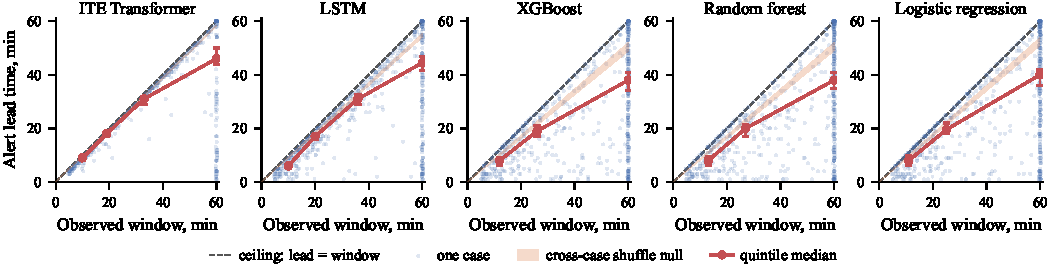
\includegraphics[width=\linewidth]{figures/Figure_A2_wide.pdf}
  \caption{\textbf{Alert lead time against observed window length, five model families, MOVER (EPIC) test.} Axes and overlays as in Figure 1. The relationship holds in every family; the transformer is the limiting case rather than the exception.}
  \label{fig:A1}
\end{figure}

\subsection{Alert composition}\label{alert-composition}

Section 5.1 reports the prevalent share as a single number per cell. For the transformer that
share is 8.7, 9.6 and 9.0\% in the three cohorts, and removing those cases moves its median lead
from 24, 17 and 22 minutes to 21, 15 and 19. Splitting detected event cases by when their first
crossing fell separates alerts that were already active at the first eligible minute from those
raised while the score was still settling and those raised later, which is the disclosure
Section 6.2's first item asks for.

\textbf{That share and Table A10's \texttt{Alerted\ by\ elapsed\ min\ 1} are different quantities rather than two
estimates of one.} The prevalent share counts detected event cases whose first crossing falls at
elapsed minute zero, the first minute of the case's own alert window, over the detected event
cases of that cell: 53 of 611, 66 of 684 and 83 of 926 for the transformer. Table A10's column
counts event cases whose first crossing falls at elapsed minute zero \textbf{or} minute one, over
every event case with a positive observed window, detected or not, as one minus the Kaplan-Meier
survival of time to first alert with each case censored at the end of its own window: 418 of 786,
463 of 1,007 and 434 of 1,409. Numerator, denominator and conditioning set all differ, and the
extra minute is the larger of the differences: minute one alone adds 365, 397 and 351 cases,
which is Section 4.1's settling read on the elapsed axis and not a second estimate of the same
immediate-alert probability. No case is censored before elapsed minute one in any of the three
cohorts, so the survival estimate at that mark equals the crude share.

\begin{figure}[H]
  \centering
  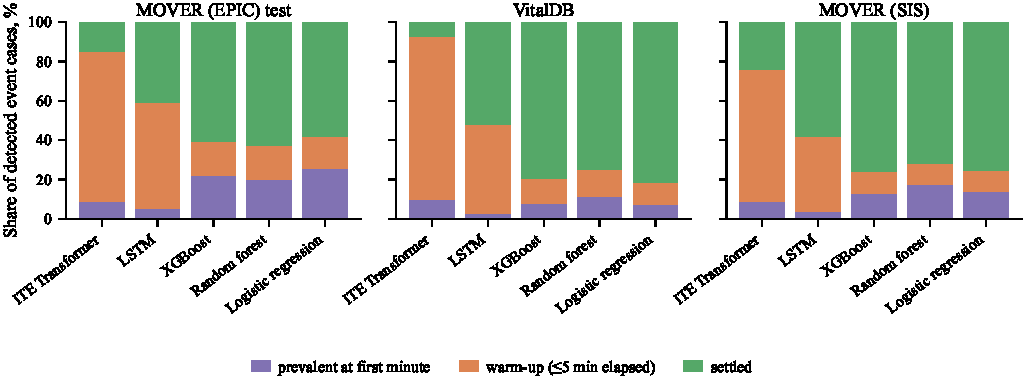
\includegraphics[width=\linewidth]{figures/Figure_3_wide.pdf}
  \caption{\textbf{Composition of detected event cases by elapsed monitoring time at the first crossing.} Prevalent cases are above threshold at their first eligible minute; warm-up cases cross within five minutes of it; settled cases cross later. Five model families, three cohorts, at the transported 80\%-sensitivity operating point. The composition differs sharply across families, in that the transformer's alerts are concentrated in the first five minutes, the LSTM's are partly so and the tabular families' are not, while the lead-to-window relationship of Section 3 holds in all of them. That is why Section 4 separates the transformer's direct mechanism from the cross-family directedness result.}
  \label{fig:A2}
\end{figure}

\subsection{Risk-set composition, and what fixing the cohort does}\label{risk-set-composition-and-what-fixing-the-cohort-does}

The population trajectory scores every case that has a minute in the bin, so its denominator
shrinks and its composition shifts as the bin moves away from onset. For an event case the
observable run-up \emph{is} its time to onset, so a short run-up is not missing data. It is an
early-onset event, and the far bins keep only the long run-ups. That is the same selection
that drives Section 3.

\textbf{Fixing the cohort moves the trajectory in both directions} (Figure A3). Recomputing the
same bins on the cases observable back to 60 minutes raises the far end and lowers the near
end, and the two curves cross at 16.4, 12.6 and 14.9 minutes before onset. The first bin
reaching AUROC 0.70 moves from 15 minutes in all three cohorts to 20, 35 and 20. Neither
curve is the true one: which denominator is used is a reporting choice, it changes the
horizon a reader would quote by up to twenty minutes, and it is not currently disclosed.
That is the whole of Section 6.2's third item.

\textbf{Short and long run-ups are different operations, which is why Section 5.3 calls this censoring
non-independent.} Splitting event cases at a 40-minute observable run-up, the long group's
operations are longer in every cohort, by a standardized mean difference of 0.394, 0.515 and
0.428, the largest imbalance on the list in all three; procedure group and ASA class are also
imbalanced beyond 0.1 in each. So a case with a short run-up is not a briefly watched version of
a case with a long one.

\begin{figure}[H]
  \centering
  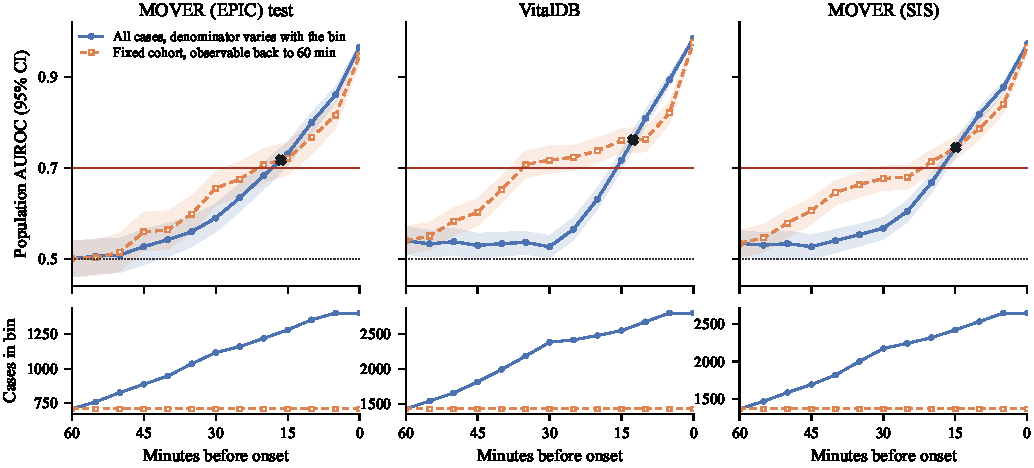
\includegraphics[width=\linewidth]{figures/Figure_A3_wide.pdf}
  \caption{\textbf{Population AUROC with its own risk set, event-aligned.} ITE Transformer, 2-minute bins from 60 minutes before onset to onset, in three held-out cohorts. Solid and filled is every case with a minute in the bin, the convention in the published literature, whose denominator varies; dashed and open is the cohort fixed to cases observable back to 60 minutes. Bands are 95\% cluster bootstrap over subjects, or over cases in MOVER (SIS). The lower row is the number of cases contributing to each bin, on its own scale per cohort. The dotted line marks 0.5, the solid rule 0.70, and the cross marks where the two curves meet.}
  \label{fig:A3}
\end{figure}

\subsection{Event and control score on the event-aligned axis}\label{event-and-control-score-on-the-event-aligned-axis}

The shape a reader expects of a continuously read score, rising in the cases that go on to
have an event and much flatter in the rest, is \textbf{present in all fifteen cells} (Figure A4).
Three things about it are worth reporting, and none is visible in a trend statistic.

\textbf{When the separation arrives runs opposite to near-onset discrimination.} For the three
tabular families the event and control means are already distinguishable 60 minutes before
onset in every cohort, the gap at that range running +0.049 to +0.109 with each pointwise
interval excluding zero. For the transformer the gap at 60 minutes \textbf{covers zero in all three
cohorts} ($-$0.023 {[}$-$0.080, 0.035{]}, $-$0.014 {[}$-$0.057, 0.030{]} and $-$0.006 {[}$-$0.043, 0.032{]}), and
first excludes it at 35, 20 and 30 minutes. The LSTM sits between the two. The family whose
scores separate latest is the one with the highest discrimination near onset.

\textbf{The event mean rises toward onset, and for the transformer the control mean falls by as
much.} Over the hour the transformer's event mean rises +0.239, +0.266 and +0.269, which is
the tendency a reader expects and it is substantial, while its control mean falls $-$0.252,
$-$0.263 and $-$0.196, so about half of the widening is carried by the controls. The LSTM's
control mean also falls, by 0.059 to 0.185. For the tabular families the control mean moves
between $-$0.070 and +0.021, rising in several cells, and the widening is almost entirely
event-side. So ``the score rises in patients who are about to have an event'' holds in every
cell here; what it leaves out is that for the transformer an equal share of the widening is
the control mean coming down, and an event-only trend statistic cannot separate the two.

\textbf{The split follows the representation more than the architecture.} The control side
contributes most where the window is read as a sequence and least where the model reads one
feature vector per scored minute, carrying each channel's last observation forward, so it sees
a level and has little shape to drift with. The ordering is not clean: the tabular families'
control means fall in MOVER (EPIC) as well and only flatten in the two external cohorts.
Representation and family are not crossed in this design, so this is a reading the data
supports rather than a hypothesis it tests. It does say where to look: \textbf{the control-side contribution is a thing
to measure in models given freer access to the input series}, and reporting the two sides of
a widening gap separately is what makes it visible.

Three things this figure is not. The control series is aligned on the sampled pseudo-onset of
Section 2 rather than on an event, so its fall is behavior over the last hour of a comparable
window and not an approach to anything. Figure A5 plots medians and this figure means, and the
two are not interchangeable here. And the two figures use different alignments: Figure A5's
axis is elapsed time from the case's first scored minute and covers the first ten minutes of
the record, where the transformer has just settled above its own 0.894 threshold, whereas the bins here
sit far later in the case, where its event mean is 0.383. \textbf{The two are not in conflict, and
the length of the plateau is what reconciles them.} The median score holds at or above the
transported threshold through elapsed minute 24, 21 and 17 in event cases and 23, 20 and 16
in controls, then falls to 0.03 to 0.31 by minute 30. Figure A5 covers the first ten of those
minutes and stops inside the plateau; every bin in this figure falls after it in all but the
shortest records.

\begin{figure}[H]
  \centering
  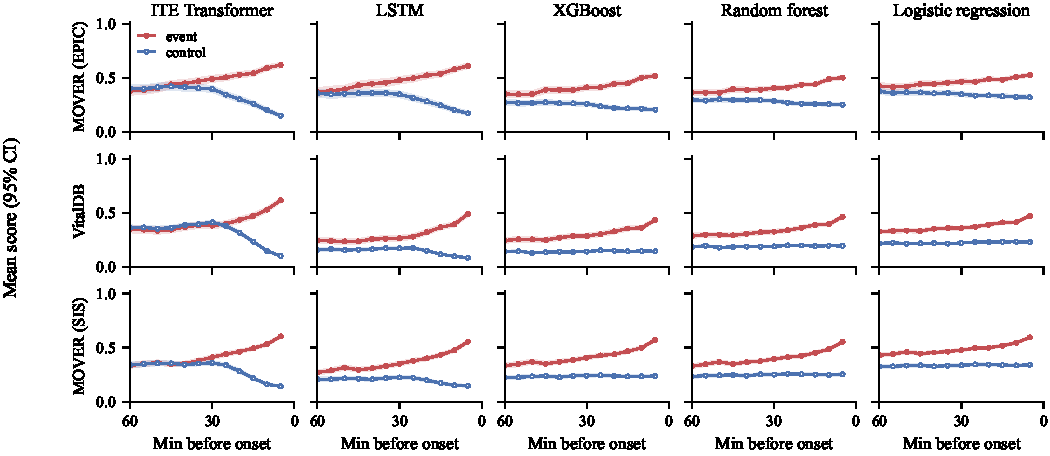
\includegraphics[width=\linewidth]{figures/Figure_A4_wide.pdf}
  \caption{\textbf{Mean score in event and control cases against minutes before onset.} Rows are cohorts, columns are model families, the same grid as Figure A5, on the event-aligned axis instead of the elapsed one. Event cases solid and filled, control cases dashed and open; bands are 95\% cluster bootstrap. Bins are the 13 centers at five-minute spacing from 60 minutes before onset; the bin at onset is empty by construction, because no minute is strictly before its own reference time, so the series ends at 5 minutes. Control cases are aligned on a sampled pseudo-onset.}
  \label{fig:A4}
\end{figure}

\subsection{Score against elapsed monitoring time}\label{score-against-elapsed-monitoring-time}

Section 4.1 reads the first ten monitored minutes of every case, and reports that the ITE
Transformer clears its own threshold there in every cohort. The margins for the others are wide.
Over those ten minutes the highest median score reached in either group is 0.69 against a
threshold of 0.78 for logistic regression in MOVER (EPIC), 0.65 against a threshold of 0.91 for
XGBoost, and 0.54 against a threshold of 0.79 for random forest. The LSTM is the one exception:
in MOVER (EPIC) it reaches 0.99 in event and 0.99 in control cases against a threshold of 0.97,
clearing it in both groups, and it clears it in neither external cohort. This is that view for
all fifteen cells, on the elapsed axis rather than the event-aligned one of Figure A4.

\begin{figure}[H]
  \centering
  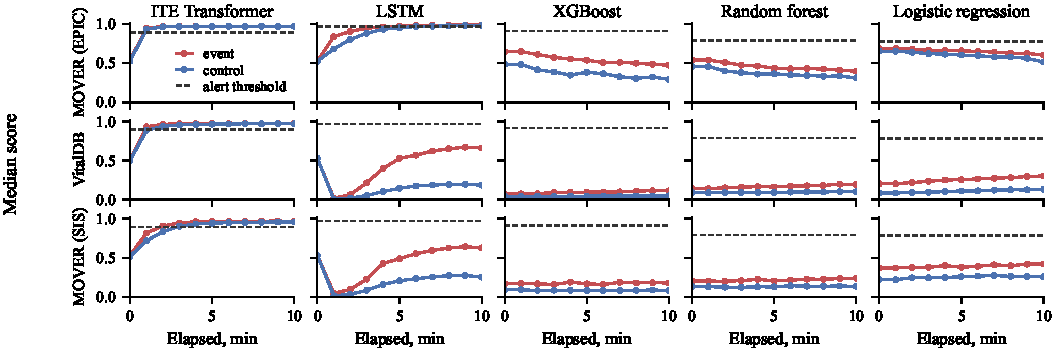
\includegraphics[width=\linewidth]{figures/Figure_1_wide.pdf}
  \caption{\textbf{Median score against elapsed monitoring time, with each family's own alert threshold.} Rows are cohorts, columns are model families. Elapsed time is measured from the case's first scored minute. The dashed rule in each panel is that family's transported raw-score threshold at the 80\%-sensitivity target, transferred unchanged from the MOVER (EPIC) validation split. Only the ITE Transformer's early rise clears its own threshold in every cohort, and it does so in event and control cases together; the LSTM does the same in MOVER (EPIC) alone. The elevation ends around minute 20, past the right edge of this axis. This axis is elapsed time; the event-aligned view is Figure A4.}
  \label{fig:A5}
\end{figure}

\subsection{Departure timing: searched for, not found}\label{departure-timing-searched-for-not-found}

We asked whether the score departs from its own baseline before mean arterial pressure
departs from its, within an episode, under a pre-specified rule: baseline is the median of
the episode's first ten eligible minutes, the robust scale is 1.4826 $\times$ the median absolute
deviation over the same minutes, and a departure is the first minute beginning a run of at
least three consecutive minutes more than 1.5 scale units in the deteriorating direction.

\textbf{Score departure does not precede MAP departure.} For XGBoost the share of episodes in
which the score departs first is significantly \emph{below} one half in all three cohorts. For the
transformer the score does not depart at all in most episodes, because its baseline sits at the
top of its range: a median baseline of 0.94 to 0.97 leaves median headroom of 0.005 to 0.031,
which is less than the bar its own rule sets in all three cohorts, so there is not enough room
above baseline for a departure to register.
Both facts are reported so the negative cannot be read as an unfair rule. Sensitivity
analyses at a 2.0 scale threshold, a five-minute run length, and a search capped at the
60-minute window all leave the direction unchanged.

The question was pre-specified and the answer constrains Section 4: whatever produces the
reported lead, it is not the score moving before the monitored variable does.

\subsection{Lead time by band, the transformer's three cohorts}\label{lead-time-by-band-the-transformers-three-cohorts}

\begin{minipage}{\linewidth}
\textbf{Table A9 \textbar{} Median alert lead time inside quantile-derived bands of observed window, ITE Transformer.} ITE
Transformer, three held-out cohorts, at the transported 80\%-sensitivity operating point.
Quintile edges are cut within each cell on detected cases; where the observed window is censored
at the 60-minute alert window the upper quintiles collapse and the realized band count is
reported rather than assumed. \texttt{Observed\ window,\ min} is the median observed pre-onset window of that band's cases rather than
an edge. Intervals are 95\% cluster bootstrap over subjects, or over cases in MOVER (SIS). All fifteen cells are Table A1; the detection rate these bands condition on is Table A5.
Section 3.1 reports the contrast this table carries.

\vspace{0.5em}
\centering\footnotesize
\begin{tabular}{@{}lrrrll@{}}
\toprule
Cohort & Band & n & Observed window, min & Median lead, min (95\% CI) & Lead / window (95\% CI) \\
\midrule
MOVER (EPIC) test & 1 & 139 & 10 & 9 {[}8, 9{]} & 0.88 {[}0.85, 0.89{]} \\
MOVER (EPIC) test & 2 & 111 & 19 & 18 {[}17, 18{]} & 0.94 {[}0.94, 0.95{]} \\
MOVER (EPIC) test & 3 & 121 & 33 & 31 {[}29, 32{]} & 0.97 {[}0.96, 0.97{]} \\
MOVER (EPIC) test & 4 & 240 & 60 & 46 {[}44, 50{]} & 0.98 {[}0.96, 0.98{]} \\
VitalDB & 1 & 143 & 7 & 5 {[}5, 6{]} & 0.83 {[}0.83, 0.83{]} \\
VitalDB & 2 & 140 & 12 & 10 {[}10, 11{]} & 0.91 {[}0.90, 0.91{]} \\
VitalDB & 3 & 132 & 20 & 19 {[}18, 20{]} & 0.94 {[}0.94, 0.95{]} \\
VitalDB & 4 & 134 & 40 & 38 {[}37, 40{]} & 0.97 {[}0.97, 0.97{]} \\
VitalDB & 5 & 135 & 60 & 59 {[}57, 60{]} & 0.98 {[}0.98, 1.00{]} \\
MOVER (SIS) & 1 & 199 & 8 & 6 {[}5, 6{]} & 0.80 {[}0.80, 0.82{]} \\
MOVER (SIS) & 2 & 179 & 17 & 14 {[}13, 15{]} & 0.86 {[}0.84, 0.91{]} \\
MOVER (SIS) & 3 & 186 & 29 & 27 {[}26, 28{]} & 0.94 {[}0.93, 0.96{]} \\
MOVER (SIS) & 4 & 362 & 60 & 46 {[}43, 49{]} & 0.95 {[}0.93, 0.97{]} \\
\bottomrule
\end{tabular}
\end{minipage}

\vspace{0.8em}

\subsection{Cohort composition and the control side}\label{cohort-composition-and-the-control-side}

\begin{minipage}{\linewidth}
\textbf{Table A10 \textbar{} Cohort composition, PPV against prevalence, and the control side.} \texttt{PPV\ $-$\ prevalence} is the lift over the base rate of the cohort the PPV is measured in, because raw PPV
is not comparable across cohorts whose prevalence runs from 0.359 to 0.560. \texttt{Alerted\ by\ elapsed\ min\ 1} is one minus the Kaplan-Meier survival of time to first alert at the first elapsed
monitoring minute, censored at the end of each case's own window; it is the censoring-aware form
of Section 4.1's settling. It is \textbf{not} the prevalent share of Section 5.1, which uses a
different numerator and a different denominator; Appendix A.11 sets the two estimands out side by
side. Intervals are 95\% cluster bootstrap.

\vspace{0.5em}
\centering\footnotesize
\begin{tabular}{@{}
  >{\raggedright\arraybackslash}p{(\columnwidth - 14\tabcolsep) * \real{0.140}}
  >{\raggedright\arraybackslash}p{(\columnwidth - 14\tabcolsep) * \real{0.110}}
  >{\raggedleft\arraybackslash}p{(\columnwidth - 14\tabcolsep) * \real{0.125}}
  >{\raggedleft\arraybackslash}p{(\columnwidth - 14\tabcolsep) * \real{0.125}}
  >{\raggedleft\arraybackslash}p{(\columnwidth - 14\tabcolsep) * \real{0.140}}
  >{\raggedleft\arraybackslash}p{(\columnwidth - 14\tabcolsep) * \real{0.140}}
  >{\raggedright\arraybackslash}p{(\columnwidth - 14\tabcolsep) * \real{0.110}}
  >{\raggedright\arraybackslash}p{(\columnwidth - 14\tabcolsep) * \real{0.110}}@{}}
\toprule
Model & Cohort & Event cases & Control cases & Prevalence & PPV $-$ prevalence & Min. above thr., controls (95\% CI) & Alerted by elapsed min 1 (95\% CI) \\
\midrule
ITE Transformer & MOVER (EPIC) test & 786 & 618 & 0.560 & +0.065 & 0.150 {[}0.050, 0.233{]} & 0.532 {[}0.497, 0.565{]} \\
ITE Transformer & VitalDB & 1007 & 1797 & 0.359 & +0.021 & 0.183 {[}0.163, 0.233{]} & 0.460 {[}0.428, 0.491{]} \\
ITE Transformer & MOVER (SIS) & 1409 & 1232 & 0.534 & +0.051 & 0.025 {[}0.017, 0.047{]} & 0.308 {[}0.285, 0.332{]} \\
LSTM & MOVER (EPIC) test & 786 & 618 & 0.560 & +0.101 & 0.017 {[}0.000, 0.027{]} & 0.228 {[}0.198, 0.257{]} \\
LSTM & VitalDB & 1007 & 1797 & 0.359 & +0.236 & 0.000 {[}0.000, 0.000{]} & 0.087 {[}0.071, 0.105{]} \\
LSTM & MOVER (SIS) & 1409 & 1232 & 0.534 & +0.151 & 0.000 {[}0.000, 0.000{]} & 0.138 {[}0.120, 0.157{]} \\
XGBoost & MOVER (EPIC) test & 786 & 618 & 0.560 & +0.165 & 0.000 {[}0.000, 0.000{]} & 0.188 {[}0.161, 0.215{]} \\
XGBoost & VitalDB & 1007 & 1797 & 0.359 & +0.253 & 0.000 {[}0.000, 0.000{]} & 0.062 {[}0.047, 0.077{]} \\
XGBoost & MOVER (SIS) & 1409 & 1232 & 0.534 & +0.180 & 0.000 {[}0.000, 0.000{]} & 0.119 {[}0.101, 0.136{]} \\
Random forest & MOVER (EPIC) test & 786 & 618 & 0.560 & +0.143 & 0.000 {[}0.000, 0.000{]} & 0.183 {[}0.157, 0.212{]} \\
Random forest & VitalDB & 1007 & 1797 & 0.359 & +0.221 & 0.000 {[}0.000, 0.000{]} & 0.101 {[}0.082, 0.121{]} \\
Random forest & MOVER (SIS) & 1409 & 1232 & 0.534 & +0.154 & 0.000 {[}0.000, 0.000{]} & 0.166 {[}0.147, 0.186{]} \\
Logistic regression & MOVER (EPIC) test & 786 & 618 & 0.560 & +0.128 & 0.000 {[}0.000, 0.017{]} & 0.226 {[}0.198, 0.255{]} \\
Logistic regression & VitalDB & 1007 & 1797 & 0.359 & +0.237 & 0.000 {[}0.000, 0.000{]} & 0.036 {[}0.025, 0.048{]} \\
Logistic regression & MOVER (SIS) & 1409 & 1232 & 0.534 & +0.152 & 0.000 {[}0.000, 0.000{]} & 0.121 {[}0.104, 0.138{]} \\
\bottomrule
\end{tabular}
\end{minipage}

\vspace{0.8em}

\subsection{What the label invites, and what the number supports}\label{what-the-label-invites-and-what-the-number-supports}

\begin{minipage}{\linewidth}
\textbf{Table A11 \textbar{} What the label invites, and what the number supports.} Column one is an affordance
of the reported label in the sense Section 1 defines, not measured comprehension. Column two is what this paper's
measurement supports in its place, and column three the disclosure that would separate them.

\vspace{0.5em}
\centering\footnotesize
\begin{tabular}{@{}
  >{\raggedright\arraybackslash}p{(\columnwidth - 4\tabcolsep) * \real{0.21}}
  >{\raggedright\arraybackslash}p{(\columnwidth - 4\tabcolsep) * \real{0.45}}
  >{\raggedright\arraybackslash}p{(\columnwidth - 4\tabcolsep) * \real{0.34}}@{}}
\toprule
What the label invites & What the number supports here & The disclosure that would close the gap \\
\midrule
The model warns about 24 minutes ahead & A median over detected event cases, itself a window-dependent set, under this cohort's window distribution (Section 3.1) & The pre-onset window distribution, and a window-conditional timing statistic (Section 6.2) \\
Twenty-four minutes is a property of the model & Within one model and cohort, median lead rises across window bands by 26 to 54 minutes, in 15 of 15 cells (Table A1) & Any single median stratified by the realized available window (Section 6.2) \\
Twenty-four minutes of usable warning & A lead read at case-level specificity 0.406, the lowest of the five families in that cohort (Table A4) & The operating point reported beside the lead (Sections 4.1, 6.3) \\
A longer lead indicates a better model & A descriptive association running the other way: lead is opposite to specificity across the fifteen combinations, Spearman $-$0.803 (Section 4.1) & Lead and operating point reported together, not lead alone (Section 6.3) \\
\bottomrule
\end{tabular}
\end{minipage}

\vspace{0.8em}

\subsection{Multiplicity}\label{multiplicity}

The two nulls of Section 3.3 form one Benjamini--Hochberg family of 75 formal tests,
adjusted within that family, of which 57 are significant at \emph{q} \textless{} 0.05. The stratification of Section 3.1 produces intervals rather than tests and does not enter the family.
Every bootstrap interval in this paper, including the fifteen window-gradient intervals of
Table A1, is a \textbf{pointwise descriptive interval}: no family-wise coverage claim is made across
the fifteen contrasts, and ``each interval excludes zero'' is fifteen separate statements rather
than one simultaneous one.

\subsection{Seeds and reproducibility}\label{seeds-and-reproducibility}

Cluster bootstraps use 2,000 replicates, with the clustering unit the subject for two cohorts
and the case for MOVER (SIS), whose released subject key is a copy of the case identifier. The
two nulls of Section 3.3 draw 1,000 permutations per cell. The cross-combination rank
correlations of Section 4.1 are reported as \textbf{point estimates with no accompanying test}. A
permutation of the pairing was computed while this analysis was being developed, and is not
reported: its unit is a cell, and cells sharing a cohort or a model family are not
exchangeable, so the resulting \emph{P} value would overstate what fifteen dependent combinations
can establish. Section 4.1 gives the untied-pair counts and the within-cohort correlations in
its place. Model training and the reference-time construction are fixed at a single seed,
reported in Appendix A.1.


% The venue's checklist guidelines require the checklist in the same PDF, after the
% references and any supplemental material, and it does not count toward the page limit.
% checklist.tex is GENERATED by make_checklist.py from the official template in
% neurips_workshop/checklist_guidelines/, so the questions and guideline blocks cannot
% drift from the shipped wording. Edit the answers in make_checklist.py, not here.
% The checklist starts on its own page.
\clearpage
\section*{NeurIPS Paper Checklist}



\begin{enumerate}

\item {\bf Claims}
    \item[] Question: Do the main claims made in the abstract and introduction accurately reflect the paper's contributions and scope?
    \item[] Answer: \answerYes{}
    \item[] Justification: The abstract and Section 1 state the four contributions and their scope. They distinguish the observed lead--window association from what the upward-biased shuffle can establish, treat low directedness as descriptive rather than causal, and state that the paper measures neither clinician comprehension nor physiology.
    \item[] Guidelines:
    \begin{itemize}
        \item The answer \answerNA{} means that the abstract and introduction do not include the claims made in the paper.
        \item The abstract and/or introduction should clearly state the claims made, including the contributions made in the paper and important assumptions and limitations. A \answerNo{} or \answerNA{} answer to this question will not be perceived well by the reviewers. 
        \item The claims made should match theoretical and experimental results, and reflect how much the results can be expected to generalize to other settings. 
        \item It is fine to include aspirational goals as motivation as long as it is clear that these goals are not attained by the paper. 
    \end{itemize}

\item {\bf Limitations}
    \item[] Question: Does the paper discuss the limitations of the work performed by the authors?
    \item[] Answer: \answerYes{}
    \item[] Justification: Section 7 is a separate limitations section covering the retrospective design, the single outcome definition, single training seed and operating-point family, the pipeline-specific results, null selection and upward bias, the single clinical domain, and the unvalidated communication and reporting proposals.
    \item[] Guidelines:
    \begin{itemize}
        \item The answer \answerNA{} means that the paper has no limitation while the answer \answerNo{} means that the paper has limitations, but those are not discussed in the paper. 
        \item The authors are encouraged to create a separate ``Limitations'' section in their paper.
        \item The paper should point out any strong assumptions and how robust the results are to violations of these assumptions (e.g., independence assumptions, noiseless settings, model well-specification, asymptotic approximations only holding locally). The authors should reflect on how these assumptions might be violated in practice and what the implications would be.
        \item The authors should reflect on the scope of the claims made, e.g., if the approach was only tested on a few datasets or with a few runs. In general, empirical results often depend on implicit assumptions, which should be articulated.
        \item The authors should reflect on the factors that influence the performance of the approach. For example, a facial recognition algorithm may perform poorly when image resolution is low or images are taken in low lighting. Or a speech-to-text system might not be used reliably to provide closed captions for online lectures because it fails to handle technical jargon.
        \item The authors should discuss the computational efficiency of the proposed algorithms and how they scale with dataset size.
        \item If applicable, the authors should discuss possible limitations of their approach to address problems of privacy and fairness.
        \item While the authors might fear that complete honesty about limitations might be used by reviewers as grounds for rejection, a worse outcome might be that reviewers discover limitations that aren't acknowledged in the paper. The authors should use their best judgment and recognize that individual actions in favor of transparency play an important role in developing norms that preserve the integrity of the community. Reviewers will be specifically instructed to not penalize honesty concerning limitations.
    \end{itemize}

\item {\bf Theory assumptions and proofs}
    \item[] Question: For each theoretical result, does the paper provide the full set of assumptions and a complete (and correct) proof?
    \item[] Answer: \answerNA{}
    \item[] Justification: The paper contains no theorems, lemmas or formal results. Its claims are empirical and each is measured on cached scores.
    \item[] Guidelines:
    \begin{itemize}
        \item The answer \answerNA{} means that the paper does not include theoretical results. 
        \item All the theorems, formulas, and proofs in the paper should be numbered and cross-referenced.
        \item All assumptions should be clearly stated or referenced in the statement of any theorems.
        \item The proofs can either appear in the main paper or the supplemental material, but if they appear in the supplemental material, the authors are encouraged to provide a short proof sketch to provide intuition. 
        \item Inversely, any informal proof provided in the core of the paper should be complemented by formal proofs provided in appendix or supplemental material.
        \item Theorems and Lemmas that the proof relies upon should be properly referenced. 
    \end{itemize}

    \item {\bf Experimental result reproducibility}
    \item[] Question: Does the paper fully disclose all the information needed to reproduce the main experimental results of the paper to the extent that it affects the main claims and/or conclusions of the paper (regardless of whether the code and data are provided or not)?
    \item[] Answer: \answerYes{}
    \item[] Justification: Yes. Two standards should be distinguished. Independent reimplementation is supported: Section 2 gives the task, cohorts, scoring policy and alert rule; Appendix A.1 gives the split sizes and seed, the eligibility rules, the twenty inputs and how each family consumes them, every architecture and training hyperparameter, and the software versions; Appendix A.19 records the seeds and resampling counts; both datasets are available under their providers' access procedures; and the analysis code is released at the anonymized repository Appendix A.1 names. Bit-for-bit reproduction from raw data is not supported here, because neither dataset may be redistributed and the cached per-minute scores the analyses read are derived patient-level data governed by the same agreements, so they are not in the repository and a reader must obtain the data themselves. We claim the first and not the second.
    \item[] Guidelines:
    \begin{itemize}
        \item The answer \answerNA{} means that the paper does not include experiments.
        \item If the paper includes experiments, a \answerNo{} answer to this question will not be perceived well by the reviewers: Making the paper reproducible is important, regardless of whether the code and data are provided or not.
        \item If the contribution is a dataset and\slash or model, the authors should describe the steps taken to make their results reproducible or verifiable. 
        \item Depending on the contribution, reproducibility can be accomplished in various ways. For example, if the contribution is a novel architecture, describing the architecture fully might suffice, or if the contribution is a specific model and empirical evaluation, it may be necessary to either make it possible for others to replicate the model with the same dataset, or provide access to the model. In general. releasing code and data is often one good way to accomplish this, but reproducibility can also be provided via detailed instructions for how to replicate the results, access to a hosted model (e.g., in the case of a large language model), releasing of a model checkpoint, or other means that are appropriate to the research performed.
        \item While NeurIPS does not require releasing code, the conference does require all submissions to provide some reasonable avenue for reproducibility, which may depend on the nature of the contribution. For example
        \begin{enumerate}
            \item If the contribution is primarily a new algorithm, the paper should make it clear how to reproduce that algorithm.
            \item If the contribution is primarily a new model architecture, the paper should describe the architecture clearly and fully.
            \item If the contribution is a new model (e.g., a large language model), then there should either be a way to access this model for reproducing the results or a way to reproduce the model (e.g., with an open-source dataset or instructions for how to construct the dataset).
            \item We recognize that reproducibility may be tricky in some cases, in which case authors are welcome to describe the particular way they provide for reproducibility. In the case of closed-source models, it may be that access to the model is limited in some way (e.g., to registered users), but it should be possible for other researchers to have some path to reproducing or verifying the results.
        \end{enumerate}
    \end{itemize}


\item {\bf Open access to data and code}
    \item[] Question: Does the paper provide open access to the data and code, with sufficient instructions to faithfully reproduce the main experimental results, as described in supplemental material?
    \item[] Answer: \answerYes{}
    \item[] Justification: The analysis code is released at an anonymized repository under the Apache License 2.0, which Appendix A.1 names, together with the aggregate result files behind every table and figure, so the table and figure checks run from the repository as shipped. The datasets are not redistributed there and cannot be: VitalDB is under a Creative Commons Attribution-NonCommercial-ShareAlike 4.0 International license and a data use agreement and MOVER is under a data use agreement, and the cached per-minute scores are derived patient-level data governed by the same agreements. Both are obtained from their own project sites once access is granted, as Appendix A.1 records, and Appendix A.1 specifies the construction to the level a reimplementation needs.
    \item[] Guidelines:
    \begin{itemize}
        \item The answer \answerNA{} means that paper does not include experiments requiring code.
        \item Please see the NeurIPS code and data submission guidelines (\url{https://neurips.cc/public/guides/CodeSubmissionPolicy}) for more details.
        \item While we encourage the release of code and data, we understand that this might not be possible, so \answerNo{} is an acceptable answer. Papers cannot be rejected simply for not including code, unless this is central to the contribution (e.g., for a new open-source benchmark).
        \item The instructions should contain the exact command and environment needed to run to reproduce the results. See the NeurIPS code and data submission guidelines (\url{https://neurips.cc/public/guides/CodeSubmissionPolicy}) for more details.
        \item The authors should provide instructions on data access and preparation, including how to access the raw data, preprocessed data, intermediate data, and generated data, etc.
        \item The authors should provide scripts to reproduce all experimental results for the new proposed method and baselines. If only a subset of experiments are reproducible, they should state which ones are omitted from the script and why.
        \item At submission time, to preserve anonymity, the authors should release anonymized versions (if applicable).
        \item Providing as much information as possible in supplemental material (appended to the paper) is recommended, but including URLs to data and code is permitted.
    \end{itemize}


\item {\bf Experimental setting/details}
    \item[] Question: Does the paper specify all the training and test details (e.g., data splits, hyperparameters, how they were chosen, type of optimizer) necessary to understand the results?
    \item[] Answer: \answerYes{}
    \item[] Justification: Appendix A.1 gives the subject-aware split and its sizes, the seed, the per-minute eligibility rules, the feature set, and for each of the five families the architecture, optimizer, learning rate, weight decay, batch size, epoch budget and early-stopping rule. Section 2 gives the calibration and threshold policy: fitted on the development validation split at an 80\% case-level sensitivity target and transported unchanged, with nothing reselected.
    \item[] Guidelines:
    \begin{itemize}
        \item The answer \answerNA{} means that the paper does not include experiments.
        \item The experimental setting should be presented in the core of the paper to a level of detail that is necessary to appreciate the results and make sense of them.
        \item The full details can be provided either with the code, in appendix, or as supplemental material.
    \end{itemize}

\item {\bf Experiment statistical significance}
    \item[] Question: Does the paper report error bars suitably and correctly defined or other appropriate information about the statistical significance of the experiments?
    \item[] Answer: \answerYes{}
    \item[] Justification: Every interval in the paper is a 95\% cluster bootstrap on the clustering unit named in Section 2, the subject for two cohorts and the case for MOVER (SIS), at 2,000 replicates; permutation nulls use 1,000 replicates and are reported as the 2.5th and 97.5th percentiles of the null distribution rather than as symmetric error bars. Appendix A.18 records the multiplicity family and its Benjamini--Hochberg adjustment, and Appendix A.19 the seeds.
    \item[] Guidelines:
    \begin{itemize}
        \item The answer \answerNA{} means that the paper does not include experiments.
        \item The authors should answer \answerYes{} if the results are accompanied by error bars, confidence intervals, or statistical significance tests, at least for the experiments that support the main claims of the paper.
        \item The factors of variability that the error bars are capturing should be clearly stated (for example, train/test split, initialization, random drawing of some parameter, or overall run with given experimental conditions).
        \item The method for calculating the error bars should be explained (closed form formula, call to a library function, bootstrap, etc.)
        \item The assumptions made should be given (e.g., Normally distributed errors).
        \item It should be clear whether the error bar is the standard deviation or the standard error of the mean.
        \item It is OK to report 1-sigma error bars, but one should state it. The authors should preferably report a 2-sigma error bar than state that they have a 96\% CI, if the hypothesis of Normality of errors is not verified.
        \item For asymmetric distributions, the authors should be careful not to show in tables or figures symmetric error bars that would yield results that are out of range (e.g., negative error rates).
        \item If error bars are reported in tables or plots, the authors should explain in the text how they were calculated and reference the corresponding figures or tables in the text.
    \end{itemize}

\item {\bf Experiments compute resources}
    \item[] Question: For each experiment, does the paper provide sufficient information on the computer resources (type of compute workers, memory, time of execution) needed to reproduce the experiments?
    \item[] Answer: \answerYes{}
    \item[] Justification: Appendix A.1 reports the hardware (one Apple M3 Ultra desktop with 512 GB unified memory, PyTorch on the Metal backend, no GPU cluster), the wall clock for each of the five models, and the fact that the project trained more than the paper reports, namely a seven-point lead-time sweep per family. The analyses in this paper add no training and read cached scores.
    \item[] Guidelines:
    \begin{itemize}
        \item The answer \answerNA{} means that the paper does not include experiments.
        \item The paper should indicate the type of compute workers CPU or GPU, internal cluster, or cloud provider, including relevant memory and storage.
        \item The paper should provide the amount of compute required for each of the individual experimental runs as well as estimate the total compute. 
        \item The paper should disclose whether the full research project required more compute than the experiments reported in the paper (e.g., preliminary or failed experiments that didn't make it into the paper). 
    \end{itemize}
    
\item {\bf Code of ethics}
    \item[] Question: Does the research conducted in the paper conform, in every respect, with the NeurIPS Code of Ethics \url{https://neurips.cc/public/EthicsGuidelines}?
    \item[] Answer: \answerYes{}
    \item[] Justification: The research conforms to the NeurIPS Code of Ethics. It is a secondary analysis of de-identified data obtained under the providers' data use agreements, with an institutional review board exemption and consent waiver recorded in Section 2 and Appendix A.1, and it proposes no model for clinical use.
    \item[] Guidelines:
    \begin{itemize}
        \item The answer \answerNA{} means that the authors have not reviewed the NeurIPS Code of Ethics.
        \item If the authors answer \answerNo, they should explain the special circumstances that require a deviation from the Code of Ethics.
        \item The authors should make sure to preserve anonymity (e.g., if there is a special consideration due to laws or regulations in their jurisdiction).
    \end{itemize}


\item {\bf Broader impacts}
    \item[] Question: Does the paper discuss both potential positive societal impacts and negative societal impacts of the work performed?
    \item[] Answer: \answerYes{}
    \item[] Justification: The paper's subject is a negative societal impact of current practice: a reported median alert lead time invites a warning-time interpretation while remaining strongly coupled to observation length, which can overstate what a deployed monitor offers. Section 5 shows that two natural repairs fail, including one whose sensitivity cost is quantified, and Section 6.2 proposes four reporting items as the mitigation. Section 7 is explicit that this is retrospective assessment and not deployment clearance.
    \item[] Guidelines:
    \begin{itemize}
        \item The answer \answerNA{} means that there is no societal impact of the work performed.
        \item If the authors answer \answerNA{} or \answerNo, they should explain why their work has no societal impact or why the paper does not address societal impact.
        \item Examples of negative societal impacts include potential malicious or unintended uses (e.g., disinformation, generating fake profiles, surveillance), fairness considerations (e.g., deployment of technologies that could make decisions that unfairly impact specific groups), privacy considerations, and security considerations.
        \item The conference expects that many papers will be foundational research and not tied to particular applications, let alone deployments. However, if there is a direct path to any negative applications, the authors should point it out. For example, it is legitimate to point out that an improvement in the quality of generative models could be used to generate Deepfakes for disinformation. On the other hand, it is not needed to point out that a generic algorithm for optimizing neural networks could enable people to train models that generate Deepfakes faster.
        \item The authors should consider possible harms that could arise when the technology is being used as intended and functioning correctly, harms that could arise when the technology is being used as intended but gives incorrect results, and harms following from (intentional or unintentional) misuse of the technology.
        \item If there are negative societal impacts, the authors could also discuss possible mitigation strategies (e.g., gated release of models, providing defenses in addition to attacks, mechanisms for monitoring misuse, mechanisms to monitor how a system learns from feedback over time, improving the efficiency and accessibility of ML).
    \end{itemize}
    
\item {\bf Safeguards}
    \item[] Question: Does the paper describe safeguards that have been put in place for responsible release of data or models that have a high risk for misuse (e.g., pre-trained language models, image generators, or scraped datasets)?
    \item[] Answer: \answerNA{}
    \item[] Justification: No model, checkpoint or dataset is released, and the paper proposes no model for clinical use, so there is nothing here with a high risk of misuse to safeguard.
    \item[] Guidelines:
    \begin{itemize}
        \item The answer \answerNA{} means that the paper poses no such risks.
        \item Released models that have a high risk for misuse or dual-use should be released with necessary safeguards to allow for controlled use of the model, for example by requiring that users adhere to usage guidelines or restrictions to access the model or implementing safety filters. 
        \item Datasets that have been scraped from the Internet could pose safety risks. The authors should describe how they avoided releasing unsafe images.
        \item We recognize that providing effective safeguards is challenging, and many papers do not require this, but we encourage authors to take this into account and make a best faith effort.
    \end{itemize}

\item {\bf Licenses for existing assets}
    \item[] Question: Are the creators or original owners of assets (e.g., code, data, models), used in the paper, properly credited and are the license and terms of use explicitly mentioned and properly respected?
    \item[] Answer: \answerYes{}
    \item[] Justification: Section 2 cites both the descriptor paper and the dataset record for VitalDB and for MOVER. Appendix A.1 names the terms: VitalDB under a Creative Commons Attribution-NonCommercial-ShareAlike 4.0 International license with a data use agreement, and MOVER free to download from the UCI Machine Learning Repository for researchers who sign its data use agreement. Software versions are listed in the same subsection.
    \item[] Guidelines:
    \begin{itemize}
        \item The answer \answerNA{} means that the paper does not use existing assets.
        \item The authors should cite the original paper that produced the code package or dataset.
        \item The authors should state which version of the asset is used and, if possible, include a URL.
        \item The name of the license (e.g., CC-BY 4.0) should be included for each asset.
        \item For scraped data from a particular source (e.g., website), the copyright and terms of service of that source should be provided.
        \item If assets are released, the license, copyright information, and terms of use in the package should be provided. For popular datasets, \url{paperswithcode.com/datasets} has curated licenses for some datasets. Their licensing guide can help determine the license of a dataset.
        \item For existing datasets that are re-packaged, both the original license and the license of the derived asset (if it has changed) should be provided.
        \item If this information is not available online, the authors are encouraged to reach out to the asset's creators.
    \end{itemize}

\item {\bf New assets}
    \item[] Question: Are new assets introduced in the paper well documented and is the documentation provided alongside the assets?
    \item[] Answer: \answerYes{}
    \item[] Justification: The analysis code is released at the anonymized repository named in Appendix A.1, under the Apache License 2.0. It carries the documentation and the aggregate result files needed to inspect and reproduce the reported tables and figures from the released artifacts. No new dataset, model or checkpoint is released, and no patient-level data are redistributed.
    \item[] Guidelines:
    \begin{itemize}
        \item The answer \answerNA{} means that the paper does not release new assets.
        \item Researchers should communicate the details of the dataset\slash code\slash model as part of their submissions via structured templates. This includes details about training, license, limitations, etc. 
        \item The paper should discuss whether and how consent was obtained from people whose asset is used.
        \item At submission time, remember to anonymize your assets (if applicable). You can either create an anonymized URL or include an anonymized zip file.
    \end{itemize}

\item {\bf Crowdsourcing and research with human subjects}
    \item[] Question: For crowdsourcing experiments and research with human subjects, does the paper include the full text of instructions given to participants and screenshots, if applicable, as well as details about compensation (if any)? 
    \item[] Answer: \answerNA{}
    \item[] Justification: No crowdsourcing was used and no participant was recruited, instructed, contacted or compensated. The work is a retrospective secondary analysis of already de-identified records.
    \item[] Guidelines:
    \begin{itemize}
        \item The answer \answerNA{} means that the paper does not involve crowdsourcing nor research with human subjects.
        \item Including this information in the supplemental material is fine, but if the main contribution of the paper involves human subjects, then as much detail as possible should be included in the main paper. 
        \item According to the NeurIPS Code of Ethics, workers involved in data collection, curation, or other labor should be paid at least the minimum wage in the country of the data collector. 
    \end{itemize}

\item {\bf Institutional review board (IRB) approvals or equivalent for research with human subjects}
    \item[] Question: Does the paper describe potential risks incurred by study participants, whether such risks were disclosed to the subjects, and whether Institutional Review Board (IRB) approvals (or an equivalent approval/review based on the requirements of your country or institution) were obtained?
    \item[] Answer: \answerYes{}
    \item[] Justification: Section 2 records that an institutional review board granted an exemption from review and waived informed consent for this secondary analysis of publicly available de-identified data, with the institution and protocol number withheld for anonymous review. Appendix A.1 records that each source collection carried its own review-board approval with consent waived after de-identification, and that this work added no data collection and no patient contact.
    \item[] Guidelines:
    \begin{itemize}
        \item The answer \answerNA{} means that the paper does not involve crowdsourcing nor research with human subjects.
        \item Depending on the country in which research is conducted, IRB approval (or equivalent) may be required for any human subjects research. If you obtained IRB approval, you should clearly state this in the paper. 
        \item We recognize that the procedures for this may vary significantly between institutions and locations, and we expect authors to adhere to the NeurIPS Code of Ethics and the guidelines for their institution. 
        \item For initial submissions, do not include any information that would break anonymity (if applicable), such as the institution conducting the review.
    \end{itemize}

\item {\bf Declaration of LLM usage}
    \item[] Question: Does the paper describe the usage of LLMs if it is an important, original, or non-standard component of the core methods in this research? Note that if the LLM is used only for writing, editing, or formatting purposes and does \emph{not} impact the core methodology, scientific rigor, or originality of the research, declaration is not required.
    %this research? 
    \item[] Answer: \answerNA{}
    \item[] Justification: No large language model is a component of the methods. The five families evaluated are a transformer over irregularly sampled physiological triplets, an LSTM, XGBoost, a random forest and logistic regression, and no LLM enters the cohort construction, the scoring policy, the alert rule or the null constructions. Generative AI was used only for English language editing of author-written text, which the policy states does not require declaration.
    \item[] Guidelines:
    \begin{itemize}
        \item The answer \answerNA{} means that the core method development in this research does not involve LLMs as any important, original, or non-standard components.
        \item Please refer to our LLM policy in the NeurIPS handbook for what should or should not be described.
    \end{itemize}

\end{enumerate}

\end{document}
